%% ----------------------------------------------------------------
%% GDP.tex
%% ---------------------------------------------------------------- 
\documentclass{ecsdocs/ecsgdp}         % Use the GDP Report Style
\graphicspath{{../Figures/}}   % Location of your graphics files
\usepackage{natbib}            % Use Natbib style for the refs.
\usepackage{array}
\usepackage{pdflscape}
\usepackage{pgfgantt}
\usepackage{pgfplots}
\usepackage{enumitem}       % For making numbered indent lists
\usepackage{color}
\usepackage{todonotes}
\usepackage{tikz}
\usetikzlibrary{automata,positioning}

\hypersetup{colorlinks=true}   % Set to false for black/white printing
%\input{Definitions}            % Include your abbreviations
\newcommand{\namedsection}[2]{\section[#1]{#1 \hfill {\small \color{gray} #2}}} % Use this to create sections with authorship: \namedsection{Section Name}{Your name}

\newcommand{\note}[1]{\todo[inline]{#1}}


%% ----------------------------------------------------------------
\begin{document}
	\frontmatter
	\title{TEST TITLE}
	\authors    {\\ \texorpdfstring
		{\href{mailto:djap1g11@ecs.soton.ac.uk}{Daniel J. A. Playle}}
		{Daniel J. A. Playle}
		\\
		\texorpdfstring
		{\href{mailto:ams2g11@ecs.soton.ac.uk}{Emily Shepherd}}
		{Emily Shepherd}
		\\
		\texorpdfstring
		{\href{mailto:mg8g12@ecs.soton.ac.uk}{Mohit Gupta}}
		{Mohit Gupta}
		\\
		\texorpdfstring
		{\href{mailto:tlf1g12@ecs.soton.ac.uk}{Toby Finch}}
		{Toby Finch}
		\\
		\texorpdfstring
		{\href{mailto:cp10g12@ecs.soton.ac.uk}{Calin Pasat}}
		{Calin Pasat}
	}
	\addresses  {\groupname\\\deptname\\\univname}
	\date       {\today}
	\subject    {}
	\keywords   {}
	\supervisor{Dr. Geoff Merrett \\ Dr. Alex Weddell}
	\examiner{Dr. Klaus-Peter Zauner}
	\degree     {Master of Engineering}
	\maketitle
	\begin{abstract}
		This work is all about \dots
	\end{abstract}
	\tableofcontents
	\listoffigures
	\listoftables
	\lstlistoflistings
	\listofsymbols{ll}
	{
		$w$ & The weight vector \\
		$S$ & The scale factor of a fixed-point number \\
		$B$ & The number of bits to shift a fixed-point number \\
	}
	%\acknowledgements{Thanks to no one.}
	%\dedicatory{To \dots}
	\mainmatter
	%% ----------------------------------------------------------------
	% Introduction chapter
	\chapter{Introduction}

Ultra-Low Power Processors, such as ARM's Cortex-M0+, are becoming an increasingly appealing area of research, particularly because they provide a platform for the Internet of Things. As our culture develops new ways for technology to aid our every-day lives, the devices which support these progressions are required to be less and less intrusive, forcing companies to search for new methods of making systems smaller and require lower power, especially as ``essentially all IoT sensor nodes will be powered by small batteries and to a lesser extent by energy harvesting'' \cite{iot_power}.

However, such processors clearly create very tight constraints for potential developers, as processing power is often limited, leading to the ever-continuing requirement for more efficient and optimised algorithms. As memory usage is also proportional to power consumption, the RAM available on such systems is extremely limiting. As we begin to rely on these systems more and more, these constraints make it a growing challenge to implement systems which are not only useful, but can be relied upon to function when needed. This is particularly important in cases in which a device is being used for safety-critical operations, which is becoming increasingly common \cite{iot_saftey} \cite{iot_saftey2}.

ARM is currently investigating the concept of a sub threshold Cortex-M0+ \cite{arm_sub}, which attempts to push the extremes of these constraints further by providing just 8 kB of memory for both program code and data, and running at just a few hundred kHz. This project aims to research and develop an algorithm which is capable of running on such a device, to act as a proof of concept that such a processor would be worthwhile.

\namedsection{Project Overview}{Finch}

The particular algorithm that the group developed is a way to identify and monitor exercises performed by a human wearer. These are specifically exercises which can be done on aeroplanes to reduce the risk of suffering from Deep Vein Thrombosis, a condition where a blood clot can form in one of the deep veins in the body, most commonly the legs. This can lead to further complications such as pulmonary embolism which occurs when part of the blood clot moves and blocks a blood vessel in the lungs \cite{dvt}. Long-haul flights can increase the risk of getting DVT because of the long periods of time sitting down and not moving which reduces circulation in the legs.

\begin{figure}[h]
  \centering
    \includegraphics[width=1.0\textwidth]{figures/exercises}
  \caption{In-flight exercises \cite{virgin2015exercises}}
  \label{fig:exercises}
\end{figure}

Figure \ref{fig:exercises} shows some of the in-flight exercises which can be performed. A few of them were looked into including the revolver, the ballerina and the shrug. These involve lifting both feet off the floor and rotating them in circles in clockwise and anticlockwise directions, pointing the feet up and down and rolling the shoulders backwards and forwards. These are all designed to help keep the circulation going in the limbs. However, a specific focus was made to the revolver exercise for the purpose of prototyping a system.

Possible uses of the algorithm would be to incorporate it into a device which could be given to passengers to strap to their legs. It would then monitor how much exercise each person was doing. This could help inform the passengers whether or not they are doing enough exercise to stay risk free. The device itself could make use of energy efficient technologies (for example the Cortex-M0+) so that its battery could easily last the entire duration of a long-haul fight.

\namedsection{Project Requirements }{Finch}

The main requirement of this project is to develop an algorithm which is capable of detecting and monitoring exercises on a sub threshold Cortex-M0+. This processor is clocked at 100 kHz, although it can increase to 3 MHz if required. However, the lower the clock speed the better as this would clearly require less power.

Additionally, 8 kB is imposed as the memory limit for both program code and data in order for the algorithm to be capable of running on the sub threshold Cortex-M0+. Again, the lower this can be the better as it opens up the possibility for the system to require even less power.

As the proposed sub threshold Cortex-M0+ is still in development, it is not readily available for the group to use; consequently, the team was required to investigate alternatives to emulate the processor. These alternatives must allow the clock speeds to be adjusted based on the efficiency and requirements of the algorithm. The challenges involved in this are discussed in chapter~\ref{chap:embedded}.

Research and analysis of the algorithms used for exercise detection which currently exist, specifically focusing on Machine Learning techniques, was also carried out. On top of this, an investigation into the tools and techniques which can be used, along with the methods by which the effectiveness of trained algorithms can be evaluated was also necessary. This is documented in chapter~\ref{chap:research}.

Following on from this, the ways in which the algorithm can be optimised to run on a such constrained system must also be explored. The way this was done is examined in chapter~\ref{chap:software}.

Another requirement of the project was to perform a user study to collect movement data of the exercises which can be used to develop the algorithm. This is so that a range of data from a selection of different people can be used because each individual is likely to perform the exercises with slight variations. The details of this can be found in chapter~\ref{chap:study}.

Finally, the accuracy of the developed algorithm is calculated; the specifics of this are outlined in chapter~\ref{chap:results}.
Below, the requirements of this project are given in explicit detail.

\namedsection{Detailed Requirements}{Finch}

\begin{enumerate}
  \item The algorithm must be capable of detecting and monitoring exercises designed to combat deep vein thrombosis
  \begin{enumerate}[label*=\arabic*.]
    \item These are exercises which can be performed in a plane, particularly in long haul flights and include:
    \begin{enumerate}[label*=\arabic*.]
      \item Foot rotations
      \item Pointing feet up and down
      \item Shoulder rolling
    \end{enumerate}
    \item Other activities such as walking should be distinguished as not being exercise
  \end{enumerate}
  \item The algorithm must be suitable to execute on an ultra-low-power sub threshold ARM Cortex-M0+
  \begin{enumerate}[label*=\arabic*.]
    \item This device has a limited processor clocked from 100 kHz to a maximum of 3 MHz
    \item Memory usage should be kept to a minimum with a target of no more than 8 kB
    \item Therefore, the algorithm should be highly optimised to use as little memory and require as little processing power as possible
  \end{enumerate}
  \item The sub threshold Cortex-M0+ must be emulated in a test platform as working with the actual M0+ is not feasible
  \begin{enumerate}[label*=\arabic*.]
    \item The test platform should be capable of being clocked at frequencies ranging from only a 100 kHz to 3 MHz
    \item The test platform should have at least 32 kB of memory to aid with testing and to act as a fall back if 8 kB cannot be achieved
    \item There must be an accelerometer sensor on the platform that readings can be taken from
  \end{enumerate}
  \item Research into various potential algorithms must take place
  \begin{enumerate}[label*=\arabic*.]
    \item Machine learning approaches should be focussed on
    \item Algorithms which are used on unconstrained systems should be considered first
    \item The feasibility of constraining those algorithms should then be investigated
    \item The methods of evaluating algorithm performance should also be examined
  \end{enumerate}
  \item Participant studies should be performed to gather movement data to train the algorithm
  \begin{enumerate}[label*=\arabic*.]
    \item Ethics approval will need to be obtained
  \end{enumerate}
  \item The developed algorithm must be deployed to the test platform
  \item The final system must then be evaluated in terms of its accuracy at detecting exercises
\end{enumerate}

	
	% Software chapter
	\chapter{Software Development}

We have discussed the requirements of the chosen algorithm, and had a detailed overview of the capabilities and limitations of the hardware available to the team. This chapter analysis's the tools and techniques used to develop such the project's algorithm, and discusses some of the trade-offs and optimisations that were investigated.

\namedsection{Developing the Algorithm}{Shepherd}

Taking into account the constraints of the system, it was decided to focus on the Multilayer Perceptron as it does not require matrix maths and typically has a smaller network of nodes. This section discusses the process by which we developed an implementation of this algorithm.

\subsection{Existing Weka Implementation \label{sec:weka-code}}

As Weka had been used to determine and train the best algorithm, it was decided to inspect its source code to obtain a starting point for the algorithm development. This, while providing a good insight into the manner in which the algorithm functions, highlighted some key areas of inefficiencies that would have to be avoided when working on a sub-threshold device.

\subsubsection{Backward Propagation}

Weka's implementation of the Multilayer Perception uses ``backward propagation'', which recursively works backwards in a depth-first manner from each output node towards the input layer. The function which calculates a node's output does so by taking the summation of each of its input values multiplied by their respective input weights. Each input value, however, is requested on the fly from the inputting node by calculating its output which in turn causes it to perform the same loop over its input nodes.

\begin{lstlisting}[language=Java,caption={Weka's method of calculating a node's output}]
class Node
{
    double weights[NUM_INPUTS];
    Node inputs[NUM_INPUTS];
    double baseValue;

    double output()
    {
        double out = base;

        for (int i = 0; i < NUM_INPUTS; i++)
        {
            out += weights[i] * inputs[i].output();
        }

        return out;
    }
}
\end{lstlisting}

A side effect of this is that all nodes, other than the output nodes are visited multiple times. For example, for the network below, $o_1.output()$ will loop over $m_1$, $m_2$ and $m_3$, calling \verb|output()| on each, each of which will loop over $i_1$, $i_2$ and $i_3$, meaning the input nodes will be visited a total of 3 times each. This process must then be repeated for $o_2$, causing the middle layer nodes to each be revisited, and the input layers revisited another 3 times, and again for $o_3$. In total each input node is accessed 9 times, the middle layer 3 times each.

\begin{figure}
    \centering
    \includegraphics{eg-ml}
    \caption{Example Multilayer Perception Network}
    \label{fig:eg-ml}
\end{figure}

Weka reduces this by storing a node's value after an \verb|output()| call. When \verb|output()| is called on a node again, it checks if it has already been called and returns the cached value if it has, as shown in listing \ref{lst:weka-cached}.

\clearpage
\begin{lstlisting}[language=Java,caption={Weka's method of preventing repeated calculations},label={lst:weka-cached}]
class Node
{
    boolean visited = false;
    double value;

    double output()
    {
        if (this.visited) return this.value;

        // Otherwise perform recursive calculation above

        this.visited = true;
        return this.value = out;
    }
}
\end{lstlisting}

While this does succeed in reducing the number of unnecessary node visits, it does not eliminate them; each node in the network, other than the output nodes, are visited three times each with this implementation. This scheme also adds two new node properties which must be stored and manipulated; the side effect of this is an increase in instructions and memory requirement, which is not ideal for sub-threshold development.

The algorithm itself still relies on recursion - this is also suboptimal as this requires extensive use of the stack. This should be avoided due to the fact the memory available on the system is very limited.

\subsubsection{The Alternative: Forward Propagation}

As a result of the inerrant inefficiencies in a Backward Propagation implementation, it was decided instead to redesign the algorithm, employing Forwards Propagation. This technique, in contrast to the one described above, starts from the input layer nodes and works forward in a breadth first manner.

For the example in figure \ref{fig:eg-ml}, this means the algorithm would first write the outputs of $i_1$, $i_2$ and $i_3$ into three memory spaces. Following this, three new memory spaces are reserved, in which the base values of $m_1$, $m_2$ and $m_3$ are placed. The algorithm then loops over the input nodes and, for each one, adds the multiplication of its value by its parent weight to the parent's memory space. Once complete, the outputs for all three middle layer nodes have been completed so the process can be shifted one layer to the right and repeated. An added benefit here is that the input layers are now no longer required, so their memory can be freed and reused if desired.

\clearpage

This method requires no stack usage and can operate in a small memory space, shown in equation \ref{eq:algo-size}. For our algorithm, which has the same number of layers as the example above, this results in only 5 32bit memory spaces: 20 bytes.

\begin{equation}
\label{eq:algo-size}
\max\{\forall L_n \in LAYERS \wedge L_{n+1} \in LAYERS : |L_n|+|L_{n+1}|\}
\end{equation}

\subsection{Moving to C Code}

During development, the team designed the C implementation to work on a desktop machine. This allowed work to focus initially on the construction of an algorithm which matched the accuracy given by Weka, without being too distracted by the finer details of embedded development, and with convenient access to debugging and \verb|stdio| tools. 

Weka is a very useful tool for generating and training machine learning algorithms. Unfortunately, it only allows exporting to \verb|.model| files, which are simply Java serialized objects. As such, Weka's source code had to be modified in order to obtain the number, structure and weightings of the nodes in the MLP's neural network.

Once the algorithm was designed, it was decided to modify and improve the Java code such that it became a harness for our C code, processing the nodes prior to output, removing unused layers and returning the required data in generated C code. This proved very useful, as training the networks and trying various settings took time and was repeated many times during development. Using this harness allowed the team to quickly deploy updated models onto the device without the need to reprogram the C code for each test.
\namedsection{Adding Heuristics}{Finch}

\note{Toby, do you wanna write this section or shall I?}
\namedsection{Developing for a Limited Environment}{Shepherd}
% This section talks about the C development

The Multilayer Perceptron is a good fit for a subthreshold Cortex M0+ as it does not require a great deal of complex mathematical computation. Unfortuneately, however, it does require the use of decimal numbers and uses the sigmoid function, which requires division and power operations. This section discusses some of the design decisions and sacrifices that were made in order to implement an MLP on the subthreshold Cortex M0+.

\subsection{Sigmoid Function}
The sigmoid function's graph and equation is shown below in figure \ref{fig:sigmoid}. Clearly, this equation causes two issues for the proposed device: firstly, it requires division, and secondly it requires the use of the constant e, which is a non-integer; using this in an operation involving powers could potentially prove expensive.

The first area of note in this graph is that the value of $f(t)$ quickly starts to tend towards 0 in the negative direction, and 1 in the positive direction. It is not uncommon, therefore, to approximate the value of the function at these extremes. Figure \ref{fig:sigmoid-ends} shows this approximation highlighted in blue for t values outside of the range between 5 and -5; it is plain to see that the error introduced here is minimal. On average, we have found that approximately 42\% \todo{REF needed} of nodes produce values in outside this range meaning they can be approximated to 0 or 1 without wasting any processing power on completing the full sigmoid function.

\begin{figure}[!h]
    \centering
    \subfigure[Normal Sigmoid Function]{\label{fig:sigmoid}\includegraphics[width=70mm]{figures/sigmoid.pdf}}
    \subfigure[Approximated Ends]{\label{fig:sigmoid-ends}\includegraphics[width=70mm]{figures/sigmoid-ends.pdf}}
    \subfigure[Approximated With Lines]{\label{fig:sigmoid-soft}\includegraphics[width=70mm]{figures/sigmoid-soft.pdf}}
    \subfigure[Approximated With Linear Equation]{\label{fig:sigmoid-hard}\includegraphics[width=70mm]{figures/sigmoid-hard.pdf}}
    \caption{Sigmoid Functions \label{fig:sigmoid-options}}
\end{figure}

For the remaining range, between 5 and -5, the sigmoid function does not tend to any fixed value, so a different approximation must be used. Fortuneately, the sigmoid's ``S''-like shape lends itself to being easily split into a series of smaller lines, as shown in figure \ref{fig:sigmoid-soft}. This provides a suitable level of accuracy with far lower computing overhead as each line can be defined using only a linar equation. However, as beneficial as the approximation in figure \ref{fig:sigmoid-soft} is, it is possible to approximate this further. We have found that approximating the sigmoid function with a single linear equation has proved satisfactory and has only lead to an observed drop in accuracy by 1\% \todo{REF}. This is shown in this section's final figure: \ref{fig:sigmoid-hard}.

\subsection{Floating point}
The lack of floating point support in the proposed device created a large challenge, as the neural network is entirely based upon a series of non-integer input weights, and the ability for each node to produce non integer output values. In order to get around this problem, the team opted for a fixed-point implementation: the weights of each node are multiplied by a scale factor and the resulting integer part is taken as the value.

This form is convienient as it makes the multiplication and addition of such scaled values straight forward: for addition of values using the same scale factor, it is sufficient to simply add the integers as though they were normal. The equation below illustrates this:

\begin{equation}
\label{eq:bits:addition}
x*S+y*S=(x+y)*S
\end{equation}

For the case of multiplation, the scale factors of each number must be added, meaning that when two numbers with a scale factor of $S$ are multiplied, the resulting number's scale factor is $S^2$:

\begin{equation}
\label{eq:bits:multiplication}
(x*S)(y*S)=(x*y)*S^2
\end{equation}

This can be easily rectified by simplying dividing the result by $S$ again to return to the original scale factor:

\begin{equation}
\label{eq:bits:rescale}
\frac{(x*y)*S^2}{S}=(x*y)*S
\end{equation}

As division is not supported on our system, we have defined our scale factor $S$ as a power of 2: $S=2^B$. We are then able to approximate divisions of powers of 2, by simply performing a bitshift:

\begin{equation}
\label{eq:bits:div_approx}
X/2^B\approx X \gg B
\end{equation}

\subsubsection{Using this on the Device}

To decide the bit scale factor, $B$, for the exercise detection algorithm, it is important to consider the memory restrictions on variable size. At a hardware level, 32bits, or 4 bytes, is the maximum size an integer can be. As the algorithm requires the multiplication of numbers, ideally these would need to fit into just a 2 bytes space, as the multiplication of numbers results in the addition of powers, as shown in equation \ref{eq:bits:multiplication-shift}.

\begin{equation}
\label{eq:bits:multiplication-shift}
(x*2^B)(y*2^B)=(x*y)*(2^B)^2=(x*y)*2^{2B}
\end{equation}

As such, the value of $B$ has to be high enough such that precision is not lost unnessisarily, but low enough such that $x*2^B<2^{16}$. Solve this, the highest possible floating point value must be known; in the case of the algorithm, this is the base value of the first node in the middle layer: -10.6 (3s.f.), using this in the rearranged equation, \ref{eq:bits:number-calc}, gives a bitshift of 12.

\begin{equation}
\label{eq:bits:number-calc}
B<\lfloor\log_{2}\left\{\frac{2^{16}}{|x|}\right\}\rfloor
\end{equation}

\subsection{Space Restrictions}

As described in \ref{section}, the device has very little memory space availiable: 8KB for both program code and data. When the algorithm code was first compiled with the mBed's precompiled libraries, the total size of the binary was 12KB. The first step to solve this was to obtain the source code for the mBed libraries; compiling these directly along with the program code, offers further potencial for the compiler to optimise the link between the API and the algorithm, based on the specific usecase.

The method was successful at reducing the total binary size to 8KB. This was a substancial improvement, however it was clear that this would need to be decreased further as it an 8KB binary leaves no space for heap or stack space when the code is run.

\subsubsection{Improving GCC's Optimisations}

While ARM's compiler is very good at optimising code when it compiles C and C++ code, the linker is not able to do so many of the same optimisations across compilation units. It was a logical first step, therefore, to identify the functions and classes that the program code calls within the mBed's api to investigate the benefits of combining their compilation unit.

In many cases, specific API calls were only made once from the algorithm code, such as the call to \verb|ic2_init()| which gets the I2C ready to communicate with the processor at the beginning of the program. Within a library, it is logical to ensure such a function remains an atomic and referenceable item, as it is feasible for a device to use more than one I2C device; as such the call may need to be made multiple times and with varying parameters.

However, as it was only called once in this case, moving \verb|ic2_init()| into the same compilation unit as the function which calls it, replacing the call with the code itself inline. As a result, the compiler is no longer required to produce assembly instructions to copy in arguments and push a new frame onto the stack; this saves not only space, but improves the performance of the code too.

\subsubsection{Argument Guards}

The mBed API's functions also often came with guards on their arguments; for example, the function \verb|gpio_init()| which is used to initialise the LED pins, accepts a pin as an arguement. Before initialising the given pin, it checks that it was not passed the pseudo-pin ``Not Connected''.

\begin{lstlisting}[caption={Argument Guards of gpio init}]
void gpio_init(gpio_t *obj, PinName pin)
{
    if (pin == (PinName)NC) // NC = Not Connected
        return;

    // gpio_init code...
}
\end{lstlisting}

Again, such a check is appropriate for an API as incorrectly passing a null pin would cause an error should the code attempt to initialise it. However, in our program we can see which pins we are passing to this function, namely the LED pins, so we can be confident that we are not passing in the null \verb|NC| pin and as such it is safe to delete the check, reducing the number of instructions required.

\subsubsection{Pinmap Functions}

The mBed library is designed to be general purpose across multiple platforms. As such the library contains a layer of abstraction to help it interface with the pins and memory addresses for a specific device. For memory addresses, this abstraction is achieved using macros in device-specific header files, which allows optimisation to can happen at compile time:

\begin{lstlisting}[caption={Memory spaces mapped in LPC11Uxx.h}]
typedef struct {                 /*!< GPIO_GROUP_INT0 Structure */
    __IO uint32_t CTRL;          /*!< GPIO grouped interrupt control register */
    __I  uint32_t RESERVED0[7];
    __IO uint32_t PORT_POL[2];   /*!< Interrupt port 0 polarity register */
    __I  uint32_t RESERVED1[6];
    __IO uint32_t PORT_ENA[2];   /*!< Interrupt port 0/1 enable register */
} LPC_GPIO_GROUP_INTx_Type;

// Peripheral memory map
#define LPC_GPIO_PIN_INT_BASE     (0x4004C000)
#define LPC_GPIO_GROUP_INT0_BASE  (0x4005C000)
#define LPC_GPIO_GROUP_INT1_BASE  (0x40060000)

#define LPC_GPIO_GROUP_INT0 ((LPC_GPIO_GROUP_INTx_Type*) LPC_GPIO_GROUP_INT0_BASE)
#define LPC_GPIO_GROUP_INT1 ((LPC_GPIO_GROUP_INTx_Type*) LPC_GPIO_GROUP_INT1_BASE)
\end{lstlisting}

The above specifices the structure of the GPIO INT memory space, then defines the memory spaces and creates references to these. This allows the developer, and the libraries to use the constant pointers, as illustrated:

\begin{lstlisting}[caption={LPC GPIO GROUP INT0 being used}]
#include ``LPC11Uxx.h'';

void main()
{
    LPC_GPIO_GROUP_INT0_BASE->CTRL = 48;
}
\end{lstlisting}

The use of these definitions allows the compiler to optimise these to constant values, as shown with the assembly below:

\begin{lstlisting}[caption={LPC GPIO GROUP INT0 converted to ASM}]
main:
    str fp, [sp, #-4]! @ Stack Init
    add fp, sp, #0     @ Stack Init
    ldr r3, .L2        @ Value of memory space
    mov r2, #48        @ Using 48
    str r2, [r3]       @ Saving 48 to the memory space
    mov r0, r3
    sub sp, fp, #0
    @ sp needed
    ldr fp, [sp], #4
    bx  lr
.L3:
    .align  2
.L2:
    .word   1074118656 @ This is 0x4005C000
\end{lstlisting}

Unfortuneately, a similar technique is not used for the Pin Mappings. Instead, these are stored in an array within a C file which is specific to each target. The values in this array are worked upon in two seperate files - one common across all devices, and one common to the device's family. The reason this is done is that the pin mappings, and the way in which their modes are updated is more complex and as such is harder to achieve through the use of defined macros. However, as the result of this is that the pin mappings and pin functions are not contained within a single compilation unit, the linker is not able to perform the same optimisations as the compiler is.

This not only results in wasted space, as the pins and their functions must be stored as part of the program code, but it also wastes valueable clock cycles, calculating values for pin addresses which could in theory be precalculated. In order to avoid this, we worked through the pin functions manually from the point at which they were called and manually calculated the registers that would be used. We then replaced these with the hard coded register values.
\namedsection{Space Restrictions \label{sec:space-restrictions}}{Shepherd}

As highlighted in section \ref{sec:cortex-limitations}, the device has very little memory space availiable: 8kB for both program code and data. When the algorithm code was first compiled with the mBed's precompiled libraries, the total size of the binary was 12kB. The first step to solve this was to obtain the source code for the mBed libraries; compiling these directly along with the program code, offers further potencial for the compiler to optimise the link between the API and the algorithm, based on the specific usecase.

The method was successful at reducing the total binary size to 8kB. This was a substancial improvement, however it was clear that this would need to be decreased further as an 8kB binary leaves no room for heap or stack space when the code is run.

\subsection{Improving GCC's Optimisations}

While ARM's compiler is very good at optimising code when it compiles C and C++ code, the linker is not able to do so many of the same optimisations across compilation units. It was a logical first step, therefore, to identify the functions and classes that the program code calls within the mBed's API to investigate the benefits of combining their compilation unit.

In many cases, specific API calls were only made once from the algorithm code, such as the call to \verb|ic2_init()| which gets the I2C ready to communicate with the processor at the beginning of the program. Within a library, it is logical to ensure such a function remains an atomic and referenceable item, as it is feasible for a device to use more than one I2C device; as such the call may need to be made multiple times and with varying parameters.

However, as it was only called once in this case, moving \verb|ic2_init()| into the same compilation unit as the function which calls it, replacing the call with the code itself inline. As a result, the compiler is no longer required to produce assembly instructions to copy in arguments and push a new frame onto the stack; this saves not only space, but improves the performance of the code too.

\subsection{Argument Guards}

The mBed API's functions also often came with guards on their arguments; for example, the function \verb|gpio_init()| which is used to initialise the LED pins, accepts a pin as an argument. Before initialising the given pin, it checks that it was not passed the pseudo-pin ``Not Connected''.

\begin{lstlisting}[caption={Argument Guards of gpio init}]
void gpio_init(gpio_t *obj, PinName pin)
{
    if (pin == (PinName)NC) // NC = Not Connected
        return;

    // gpio_init code...
}
\end{lstlisting}

Again, such a check is appropriate for an API as incorrectly passing a null pin would cause an error should the code attempt to initialise it. However, in our program we can see which pins we are passing to this function, namely the LED pins, so we can be confident that we are not passing in the null \verb|NC| pin and as such it is safe to delete the check, reducing the number of instructions required.

\subsection{Device-Specific Memory Mapping}

The mBed library is designed to be general purpose across multiple platforms. As such the library contains a layer of abstraction to help it interface with the pins and memory addresses for a specific device.

\subsubsection{Ideal Memory Mapping}\label{section:constant-memory-map}

For memory addresses, this abstraction is achieved using macros in device-specific header files, which allows optimisation to can happen at compile time:

\begin{lstlisting}[caption={Memory spaces mapped in LPC11Uxx.h}]
typedef struct {                 /*!< GPIO_GROUP_INT0 Structure */
    __IO uint32_t CTRL;          /*!< GPIO grouped interrupt control register */
    __I  uint32_t RESERVED0[7];
    __IO uint32_t PORT_POL[2];   /*!< Interrupt port 0 polarity register */
    __I  uint32_t RESERVED1[6];
    __IO uint32_t PORT_ENA[2];   /*!< Interrupt port 0/1 enable register */
} LPC_GPIO_GROUP_INTx_Type;

// Peripheral memory map
#define LPC_GPIO_PIN_INT_BASE     (0x4004C000)
#define LPC_GPIO_GROUP_INT0_BASE  (0x4005C000)
#define LPC_GPIO_GROUP_INT1_BASE  (0x40060000)

#define LPC_GPIO_GROUP_INT0 ((LPC_GPIO_GROUP_INTx_Type*) LPC_GPIO_GROUP_INT0_BASE)
#define LPC_GPIO_GROUP_INT1 ((LPC_GPIO_GROUP_INTx_Type*) LPC_GPIO_GROUP_INT1_BASE)
\end{lstlisting}

The above specifies the structure of the GPIO INT memory space, then defines the memory spaces and creates references to these. This allows the developer, and the libraries to use the constant pointers, as illustrated:

\begin{lstlisting}[caption={LPC GPIO GROUP INT0 being used}]
#include ``LPC11Uxx.h'';

void main()
{
    LPC_GPIO_GROUP_INT0_BASE->CTRL = 48;
}
\end{lstlisting}

The use of these definitions allows the compiler to optimise these to constant values, as shown with the assembly below:

\begin{lstlisting}[caption={LPC GPIO GROUP INT0 converted to ASM}]
main:
    str fp, [sp, #-4]! @ Stack Init
    add fp, sp, #0     @ Stack Init
    ldr r3, .L2        @ Value of memory space
    mov r2, #48        @ Using 48
    str r2, [r3]       @ Saving 48 to the memory space
    mov r0, r3
    sub sp, fp, #0
    @ sp needed
    ldr fp, [sp], #4
    bx  lr
.L3:
    .align  2
.L2:
    .word   1074118656 @ This is 0x4005C000
\end{lstlisting}

\subsubsection{Inefficient Mapping}

Unfortunately, a similar technique is not used for the Pin Mappings. Instead, these are stored in an array within a C file which is specific to each target, as shown below. These values are worked upon in two separate files - one common across all devices, and one common to the device's family.

\begin{lstlisting}[caption={PinMap Arrays}]
const PinMap PinMap_UART_TX[] = {
    {P0_19, UART_0, 1},
    {P1_13, UART_0, 3},
    {P1_27, UART_0, 2},
    { NC  , NC    , 0}
};

const PinMap PinMap_UART_RX[] = {
    {P0_18, UART_0, 1},
    {P1_14, UART_0, 3},
    {P1_26, UART_0, 2},
    {NC   , NC    , 0}
};
\end{lstlisting}

The reason for this is that the library is used to support a wide range of devices and configurations; the number of peripherals from use to use, and the way in which these are connected up by specific users, is entirely unpredictable, and leads to a more complex mapping structure being required. This is harder, and sometimes not possible, to achieve through the use of defined macros.

This not only results in wasted space, as the pins and their functions must be stored as part of the program code, but it also wastes valuable clock cycles, calculating values for pin addresses which could in theory be pre calculated. \verb|i2c_init()|, for example, first loops over the PinMap to find the memory address for the I2C with its SDA connected on pin 28, then repeats this process to search for the I2C with its SCL pin on port 27. Finally, it checks that these I2Cs are the same, before saving this memory address to a pointer for actual use. In total, this requires 5 function calls, and uses two loops to search over the data-mapping array; none of this can be optimised as it is spread across multiple compilation units. Setting just these two pin's mode and function requires a further 8 function calls, and 4 loops over the PinMap data structure.

It is plain to see that this is an extremely inefficient process and requires superfluous instructions to be added to the binary, especially as the device used for this project, the \verb|LPC11U24_401|, can have only one I2C bus and as such these functions can only ever return the same memory address each and every time they are run. In order to avoid this, these constant memory addresses were calculated by hand then saved in the form of a defined macro as used in the section above. The entirety of the pinmap data structure and supporting functions could then be removed from the project, drastically reducing its memory footprint.

\subsection{General Library Overhead}

A secondary side effect of using libraries is that they come with a large amount of general overhead; for example, the gyroscopic device that was used, the \verb|MPU6050| comes with a C++ class to interact with it. This, in turn, used its own secondary class, \verb|I2Cdev|, to interact with the device over the I2C bus. This class contained the logic to transform values into bit masks to allow the updating of individual bits within the device's configuration registers. These bit masks were passed on to the mBed library's \verb|I2C| class, which holds a \verb|struct| containing the pointer to the I2C memory address range, and acts as a wrapper for the mBed library's C I2C functions.

Defining, instantiating and storing a pointer, within a struct, within a class, within a class, within yet another class is an enormous overhead, especially as the middle layers of this abstraction are not adding significant functionality, but are merely acting as gatekeepers between the \verb|MPU6050| class and the lower level I2C functions. As part of the optimisation process, these unnecessary data structures were combined and removed where possible: pointers to memory addresses were replaced with definitions, as discussed above in section \ref{section:constant-memory-map}, bit masks were replaced with precomputed constants, and the MPU class was converted into a set of static functions to be called directly from \verb|main()|, removing the need to instantiate an object at all.


	\namedsection{Exercise Detection}{Daniel Playle}
% This section discusses the exercise detection aspects of the software
% You can probably see where this is going...
% Blah blah can do exercise detection with X
% Blah blah can use machine learning
% Papers A, B and C use machine learning
% Machine learning is good, use machine learning

	% Exercise detection is required
	% Several methods of detecting exercise
	% 
	
	Exercise detection is a key aspect of the of the project, and a focus on foot exercises was required. 
	\namedsection{Machine Learning}{Playle}
\label{ml}

%%%%%%%%%%%%%%%%%%%%%%%%%%%%%%%%%
%%% WHAT IS MACHINE LEARNING? %%%
%%%%%%%%%%%%%%%%%%%%%%%%%%%%%%%%%
Machine learning is a technique that takes some observations about a system in addition to a value of interest \todo{Maybe s/value of interest/output/}, builds a model around these parameters and uses this model to create predictions about the value of interest for the system. There are typically three categories of machine learning algorithm: classification, where the value of interest is in a finite set of classes; regression, where the value of interest is continuous; and clustering, where the value of interest is related to other values.

In order to detect exercise, a classifying supervised machine learning algorithm will be most suitable, with the classes being types of activity observed.

\subsection{Considered Issues}

%%%%%%%%%%%%%%%%%%%%%%%%%%%%%%%
%%% CURSE OF DIMENSIONALITY %%%
%%%%%%%%%%%%%%%%%%%%%%%%%%%%%%%
One of the frequently encountered problems is the curse of dimensionality \cite{bellman1957dynamic}. Having a high number of dimensions, often as a result of having a large number of inputs into a machine learning algorithm, can create the problem whereby the amount of instances required to sufficiently train the model increases as the amount of training of the model must have instances such that the input feature space must be explored sufficiently. \cite{oommen2008objective}. Further to this effect, the time and space complexity of many machine learning algorithms are functions of the feature space's dimensionality. However, existing work has demonstrated that the curse of dimensionality is not necessarily applicable to time-series data as the nature of such data explores the feature space on the condition that the signal-to-noise ratio is sufficiently high \cite{bernecker2011quality}.

%%%%%%%%%%%%%%%%%%%
%%% OVERFITTING %%%
%%%%%%%%%%%%%%%%%%%
\todo{cites}
Another problem encountered in machine learning is that of overfitting, where the model for some algorithm is trained such that it specialises on the training set alone. This can be problematic where the model is introduced to new data, as such models have poor performance on unseen data. Overfitting can be prevented by reducing the complexity of the model, as if the model is not complex enough, it is not possible for it to overfit on the training data exactly. Additionally, evaluation should be performed on a data set other than the training set, which can be achieved with using cross-validation, or even having a completely separate data set on which to test.

\note{How exactly does the machine learning algorithm work? Reference papers that describe these methods.}

\note{What experiments were conducted in order to determine machine learning feasibility?}
\subsection{Initial Feasibility Assessment}
In order to initially determine the feasibility of applying machine learning for detecting exercise, a simple experiment was conducted with a single subject. The intent of the experiment was to implement a similar machine learning algorithm as is described in \cite{kwapisz2011activity} to ensure understanding of the problem at hand.

The collection device used came in the form of a Sony Z3 mobile phone, providing kinematic sensors, of which the gyroscope, measuring the angular velocity, was used. The subject had the collection device attached to their foot while they performed activities including a foot rotation exercise; walking on a flat surface; and walking up and down stairs. Additionally, noise was collected by moving the collection device in random directions. The collection device sampled data at 200Hz on each axis, so for the purpose of assessing feasibility, this value was carried through into machine learning, using a window size of 200 samples for a classification over 1 second intervals.

Data for each activity was collected separately to ensure classification could be performed without having to note exact timings of activities. Some examples of the data collected in these activities are shown in figure \ref{fig:first-data}, where the periodic nature of all the activities (with the exception of noise), can be seen clearly. \todo{Discuss this data more?}

This data was run through a series of tools to build a model, as described in section \ref{sec:tools-produced}. Initial evaluation of the performance was conducted using 10-fold cross-validation. The confusion matrix for a simple naive Bayes classifier is shown in table \ref{tab:first-confusion}, giving a classification accuracy of \todo{}. Despite the data only being collected from a single individual using a small set of instances, the results were promising, indicating that machine learning as a method of activity recognition was feasible.

\begin{table}[]
	\centering
	\begin{tabular}{|cccc|ll|}
		\hline
		\multicolumn{4}{|c|}{Classified As}   &          &                        \\
		Exercise & Noise & Stairs & Walking &          &                        \\
		\hline
		62       & 0     & 0      & 0       & Exercise & \multirow{4}{*}{Class} \\
		2        & 15    & 1      & 0       & Noise    &                        \\
		3        & 0     & 10     & 3       & Stairs   &                        \\
		1        & 0     & 1      & 7       & Walking  &                       \\
		\hline
	\end{tabular}
	\caption{Feasibility Assessment Confusion Matrix \label{tab:first-confusion}}
\end{table}


\begin{figure}
	\centering
	\subfigure[Exercise]{\label{fig:first-exercise}\includegraphics[width=70mm]{figures/first-exercise.pdf}}
	\subfigure[Noise]{\label{fig:first-noise}\includegraphics[width=70mm]{figures/first-noise.pdf}}
	\subfigure[Stairs]{\label{fig:first-stairs}\includegraphics[width=70mm]{figures/first-stairs.pdf}}
	\subfigure[Walking]{\label{fig:first-walking}\includegraphics[width=70mm]{figures/first-walking.pdf}}
	\caption{Feasibility Assessment Data \label{fig:first-data}}
\end{figure}

%%%%%%%%%%%%%%%%%%%%%%%%%%%%%
%%% TOOLS USED / PRODUCED %%%
%%%%%%%%%%%%%%%%%%%%%%%%%%%%%
\subsection{Tools \label{sec:tools}}
Weka, a machine learning library, was used extensively for machine learning aspects. It provides a vast multitude of implemented machine learning algorithms, including various methods of evaluating the performance of these trained models.

%%%%%%%%%%%%%%%%%%%%%%%
%%% THE ARFF SCRIPT %%%
%%%%%%%%%%%%%%%%%%%%%%%
In order to produce this, it is first necessary to know the desired classification over given intervals for some time series data. This is achieved by mapping a single point of interest on some time series data to a class. This mapping is then passed to a script that takes windows centered on these points of interest and creates the corresponding \texttt{.arff}. In addition to these points of interest, the number of samples per window is also taken.

%%%%%%%%%%%%%%%%%%%%
%%% DOWNSAMPLING %%%
%%%%%%%%%%%%%%%%%%%%
Data collection is already an expensive task in terms of time consumed. It was therefore deemed infeasible to sample at multiple frequencies on top of all the variables being explored during data collection. Further to this, the device being used for data collection was rigid in terms of allowable sampling frequencies. To allow for analysis of multiple sampling frequencies at a later data, sampling was done at 200Hz, the fastest the collection device would allow. Any collected data could then be downsampled, which was achieved by taking the closest sample to $n/f$ where f is the frequency to downsample to.

%%%%%%%%%%%%%%%%%%%%%%
%%% CLASSIFICATION %%%
%%%%%%%%%%%%%%%%%%%%%%
As shown in figure \ref{fig:first-data}, activities produce periodic data that is easily manually identified. This feature of the collected data was used to in order to identify the intervals for classification. Collected data was separated at the time of collection into individual files each representing a different activity/sensor tuple, allowing for trivial manual classification.

The act of data classification occurred by viewing the plotted data and points of interest were noted. For the two exercise classes \todo{Name the classes?}, the points of interest were the peak and trough of the y-axis. For the class representing not exercise, points of interest were taken at frequent points throughout collected data files where subjects were not performing exercise, meaning that manual classification of the not exercise class was not required.

These classified points of interest were then run through a script 

%%%%%%%%%%%%%%%%%%%%%%%%%%%%%%%%%%%
%%% ASSESSING MODEL PERFORMANCE %%%
%%%%%%%%%%%%%%%%%%%%%%%%%%%%%%%%%%%
There are multiple methods of assessing the performance of a model. A simple assessment may include measuring the accuracy, although this does not take into account the probability of specific classes existing, and can therefore skew results when there are significantly more instances of a subset of classes over another subset of classes. An extreme example of this is the 0-R classifier, which will determine the most frequent class and classify all instances as this. Such a classifier is very simple, and has a severely limited utility, but as shown in \todo{figure}, a high accuracy is still possible, despite what can be considered poor performance.

By taking into account the probability of classes existing, the bias that leads to this poor metric can be eliminated. Such a statistic is the kappa statistic \todo{add cite}, which measures performance with respect to a null classifier, that is, a classifier that solely takes into account the frequencies of observed data. A kappa statistic, $\kappa < 0$  would indicate very bad performance (worse than guessing while taking into account the class frequencies). $\kappa$ increasing from 0 to 1 indicates increasing performance, with $\kappa = 1$ being a perfect classifier. The kappa statistic has therefore been used to measure the performance of later classifiers.

% Maybe remove this
In some cases, it may be important to quantify the trade-off a classifier makes between true and false positives. This can especially be the case where it is more important to detect some class over another. Achieving this can be done with a custom cost function, which is applied to the resultant confusion matrix (equation \ref{eq:cost}). From this, the average cost per instance can be computed, allowing comparisons to be drawn.

\begin{equation}
	\label{eq:cost}
	\begin{gathered}
		\text{Cost } c = \langle \mathbf{COST}, \mathbf{CONFUSION} \rangle_F \\
		\text{Where $\langle \mathbf{A}, \mathbf{B}\rangle_F$ is the Frobenius inner product between $\mathbf{A}$ and $\mathbf{B}$}
	\end{gathered}
\end{equation}

This method of performance quantification is similar to an ROC curve, except where 

Weka accepts instances in the form of an \texttt{.arff} file, this file specifies all the classes for the classifier to accept; the inputs for the classifier; and some number of instances and their actual class, if known.


%%%%%%%%%%%%%%%%%%%%%%%%%%%%%
%%% 3 CLASSES OVER JUST 2 %%%
%%%%%%%%%%%%%%%%%%%%%%%%%%%%%
The number of classes to classify was considered, as a variable parameter for the classifier. A classifier with the 2 classes \textit{exercise} \todo{Maybe s/exercise/activity/} and \textit{not exercise}, would only allow for binary classification. Depending on the classifier behaviour and the nature of the exercise in question, it may be the case that when the window of classification lies between 2 exercises, the window could be classified as either class. This unpredictable behaviour would prevent further analysis of the subject's exercise beyond how much time exercise has been detected for. \todo{Add figure}. However, by splitting the \textit{exercise} class into 2 distinct classes, such that every exercise performed will always be composed of these parts, it allows 3 classes to be used with the classifier. Such a change would allow counting of distinct exercises, by ensuring that one type of \textit{exercise} class is followed by the other type of \textit{exercise} class. This would allow the number of exercises to be counted, as well as the amount of time exercised. Further to this, the additional information may allow for heuristics to increase accuracy should the classifier ``bounce''. \todo{More on this in heuristics...} Other numbers of classes were also considered, such as some number of classes for the exercise, along with a class for each likely type of non-exercise activity. \todo{and this idea was rejected because...}

\note{What classification algorithms were trialled? What kind of results were achieved with these. Explain and discuss the workings of each algorithm / type of algorithm.}

\subsection{Multilayer Perceptrons}
A Multilayer Perceptron (MLP) is a type Neural Network, where the nodes, or perceptrons, are organised in layers. Each node accepts some number of inputs with some weight. These summation of these weighted inputs are computed and applied to some activation function, the result of which is the output of the node (equation \ref{eq:perceptron}).

\begin{equation}
\label{eq:perceptron}
\text{Output } o = activation\bigg(\sum_{i=1}^{d}{x_iw_i}\bigg) 
\end{equation}

Each perceptron affectively defines a plane in $d$-dimensional space. Instances on either side of this plane can then be classed, allowing a single perceptron to act as a simple classifier. By combining multiple perceptrons in a layer, it is possible to build up these planes in order to create more complex classifier made of these linear classifiers. The addition of layers, using previous layers are inputs allows a more complex classifier still by allowing the importance of these sub-classifiers to vary with the inputs. MLPs with enough inputs and layers can therefore replicate any function \cite{baum1988capabilities}.

\note{Finish/tidy this and wrap in figure}
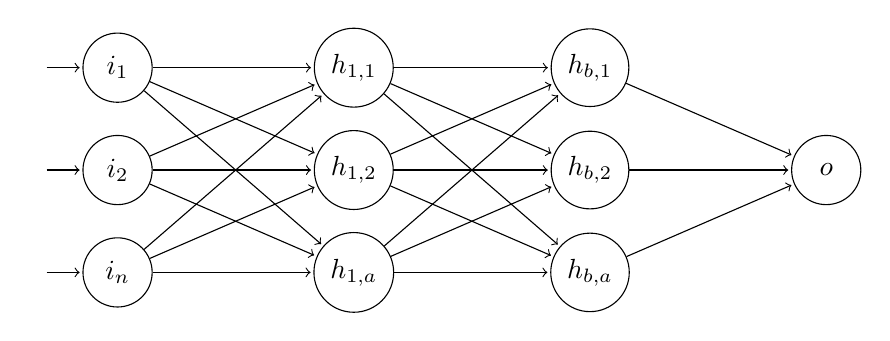
\begin{tikzpicture}[shorten >=1pt,node distance=1.3cm and 3cm,on grid,auto,initial text={}] 
\node[state,initial] (i1) {$i_1$};
\node[state,initial] (i2) [below=of i1] {$i_2$}; 
\node[state,initial] (in) [below=of i2] {$i_n$}; 

\node[state] (h11) [right=of i1] {$h_{1,1}$};
\node[state] (h12) [below=of h11] {$h_{1,2}$}; 
\node[state] (h1a) [below=of h12] {$h_{1,a}$}; 

\node[state] (hb1) [right=of h11] {$h_{b,1}$};
\node[state] (hb2) [below=of hb1] {$h_{b,2}$}; 
\node[state] (hba) [below=of hb2] {$h_{b,a}$}; 

\node[state] (o) [right=of hb2] {$o$};
\path[->] 
(i1) edge node {} (h11) (i2) edge node {} (h11)
(i1) edge node {} (h12) (i2) edge node {} (h12)
(i1) edge node {} (h1a) (i2) edge node {} (h1a)
(in) edge node {} (h11) (h11) edge node {} (hb1)
(in) edge node {} (h12) (h11) edge node {} (hb2)
(in) edge node {} (h1a) (h11) edge node {} (hba)
(h12) edge node {} (hb1) (h1a) edge node {} (hb1)
(h12) edge node {} (hb2) (h1a) edge node {} (hb2)
(h12) edge node {} (hba) (h1a) edge node {} (hba)

(hb1) edge node {} (o)
(hb2) edge node {} (o)
(hba) edge node {} (o)
;
\end{tikzpicture}

\subsection{Radial Basis Function Networks}
A Radial Basis Function (RBF) network is a type of Neural Network that is composed of 2 layers, an input layer and an output layer. The activation functions for this output layer are RBFs. An RBF can be any function that is only dependent on the distance from some point. An example of a commonly used RBF is the Gaussian function.

\subsection{Instance-Based Learning}
Instance-based learning is a type of machine learning algorithm that postpones model creation until an output for a problem instance is required. Some number of labelled instances are stored in memory, and these are used to label problem instances.

Instance-based learning is advantageous over other machine learning methods in that adapting the model with new instances is trivial. This makes it attractive for simple systems where some adaptation of the model is required.

As a number of labelled instanced must be kept in memory in order to compute the model, instance-based learning methods can require large amounts of memory to classify. Additionally, any problem instances must be compared against each labelled instanced that is to be used for the model, meaning that time complexity for classification of any problem instance is linear in the number of labelled instances. This can present significant challenges when the size of the training data set become large with respect to the underlying device.

An example of instance-based learning is the k-nearest neighbours algorithm where any problem instance is compared to the k-nearest labelled instances. The class that the problem instance is most similar to is then given this classification. \todo{Reword}

\note{What issues were faced as a result of implementing a machine learning algorithm on a constrained system? How were these problems overcome? \cite{anguita2012human}}
Each machine learning algorithm comes with its own memory-processing-accuracy trade-off, 

%%%%%%%%%%%%%%%%%%%%%%%%%%%%
%%% ALGORITHM PARAMETERS %%%
%%%%%%%%%%%%%%%%%%%%%%%%%%%%
\note{Selection of the algorithm - mention hidden layers  /frequency}
There are many parameters that affect the performance of classifiers. In the case of the collected data, the sampling frequency for the kinematic sensor and the window with a number of samples over which the classifier classifies have a direct impact on the classifier's ability to perform. In the case of the model, most machine learning algorithms have some form parameters allowing their behaviour to change. 

As the MLP was 

%%%%%%%%%%%%%%%%%%%%%%%%%%
%%% USER STUDY RESULTS %%%
%%%%%%%%%%%%%%%%%%%%%%%%%%
\subsection{User Study Results}
\note{As a result of the user study, how did the results change? Note observed results due to the user study.}
The user study was performed on a number \todo{How many?} subjects, where both accelerometer and gyroscope data was collected for multiple activities.

%%%%%%%%%%%%%%%%%%%%%%%%%%%
%%% ALGORITHM SELECTION %%%
%%%%%%%%%%%%%%%%%%%%%%%%%%%
The main contenders for the algorithm were the MLP and RBF network due to high performance while having relatively low complexity, allowing them to be implemented on a constrained device without too much difficulty. Between these two algorithms, there was minimal difference in terms of 

\begin{figure}
	\centering
	\subfigure[Top-Down]{\label{fig:mlp-multi-flat}\includegraphics[width=70mm]{figures/mlp-multi-analysis-flat.pdf}}
	\subfigure[Side-On, Varying Hidden Layers]{\label{fig:mlp-multi-3d}\includegraphics[width=64mm]{figures/mlp-multi-analysis-3d.pdf}}
	%\subfigure[Varying Frequency]{\label{fig:mlp-multi-3d-2}\includegraphics[width=70mm]{figures/mlp-multi-analysis-3d-2.pdf}}
	%\subfigure[Varying Both]{\label{fig:mlp-multi-3d-3}\includegraphics[width=70mm]{figures/mlp-multi-analysis-3d-3.pdf}}
	\caption{MLP Parameter Performance Surface Plot \label{fig:mlp-multi}}
\end{figure}

\begin{figure}
	\includegraphics[width=\linewidth]{subject-fold-results.pdf}
	\caption{Subject Performance with Different Sensors and Algorithms \label{fig:subfold}}
\end{figure}
% Note: acc-mlp 0.5842176471 (-)
%       acc-rbf 0.6203764706 (tt 0.6053772895)
%       gyr-mlp 0.6116235294 (tt 0.5858137193)
%       gyr-rbf 0.8015705882 (tt 0.0002064496) <-- Mention this

%%%%%%%%%%%%%%%%%%%%%%%%%%%%%%%%%%%
%%% WHY CROSS-VALIDATION IS BAD %%%
%%%%%%%%%%%%%%%%%%%%%%%%%%%%%%%%%%%
To evaluate the models on the user study data, cross-validation was considered, as this would allow training on some set of data and then testing on another set previously unseen to the model, although this would have the slightly undesirable effect of mixing data from subjects, whereas in practice, the device will be trained on a set of subjects and used by a subject not in that set. To replicate this kind of behaviour, a similar method to cross-validation was used, where the model was trained on all subjects, except for one. This one excluded subject was then tested on. This method is then repeated for all subjects. This subject-fold cross-validation method is also beneficial in allowing conclusions to be drawn about subject performance in relation to other subjects.

A noteworthy observation about the results was that the performance of the algorithm was initially poor, by any measure, after the first day data collection, giving just 5 \todo{Really?} subjects to model against. However, as the number of subjects increased, so did the performance of the system. This would indicate that the algorithm was overfitting on subjects, and that the introduction of more subjects was able to at least in part negate this overfitting.

\note{What parameters are there and how did they affect the accuracy of the system?}

\note{Still need to add RBF stuff...}
	\namedsection{Developing for a Limited Environment}{Shepherd}
% This section talks about the C development

The Multilayer Perceptron is a good fit for a subthreshold Cortex M0+ as it does not require a great deal of complex mathematical computation. Unfortuneately, however, it does require the use of decimal numbers and uses the sigmoid function, which requires division and power operations. This section discusses some of the design decisions and sacrifices that were made in order to implement an MLP on the subthreshold Cortex M0+.

\subsection{Sigmoid Function}
The sigmoid function's graph and equation is shown below in figure \ref{fig:sigmoid}. Clearly, this equation causes two issues for the proposed device: firstly, it requires division, and secondly it requires the use of the constant e, which is a non-integer; using this in an operation involving powers could potentially prove expensive.

The first area of note in this graph is that the value of $f(t)$ quickly starts to tend towards 0 in the negative direction, and 1 in the positive direction. It is not uncommon, therefore, to approximate the value of the function at these extremes. Figure \ref{fig:sigmoid-ends} shows this approximation highlighted in blue for t values outside of the range between 5 and -5; it is plain to see that the error introduced here is minimal. On average, we have found that approximately 42\% \todo{REF needed} of nodes produce values in outside this range meaning they can be approximated to 0 or 1 without wasting any processing power on completing the full sigmoid function.

\begin{figure}[!h]
    \centering
    \subfigure[Normal Sigmoid Function]{\label{fig:sigmoid}\includegraphics[width=70mm]{figures/sigmoid.pdf}}
    \subfigure[Approximated Ends]{\label{fig:sigmoid-ends}\includegraphics[width=70mm]{figures/sigmoid-ends.pdf}}
    \subfigure[Approximated With Lines]{\label{fig:sigmoid-soft}\includegraphics[width=70mm]{figures/sigmoid-soft.pdf}}
    \subfigure[Approximated With Linear Equation]{\label{fig:sigmoid-hard}\includegraphics[width=70mm]{figures/sigmoid-hard.pdf}}
    \caption{Sigmoid Functions \label{fig:sigmoid-options}}
\end{figure}

For the remaining range, between 5 and -5, the sigmoid function does not tend to any fixed value, so a different approximation must be used. Fortuneately, the sigmoid's ``S''-like shape lends itself to being easily split into a series of smaller lines, as shown in figure \ref{fig:sigmoid-soft}. This provides a suitable level of accuracy with far lower computing overhead as each line can be defined using only a linar equation. However, as beneficial as the approximation in figure \ref{fig:sigmoid-soft} is, it is possible to approximate this further. We have found that approximating the sigmoid function with a single linear equation has proved satisfactory and has only lead to an observed drop in accuracy by 1\% \todo{REF}. This is shown in this section's final figure: \ref{fig:sigmoid-hard}.

\subsection{Floating point}
The lack of floating point support in the proposed device created a large challenge, as the neural network is entirely based upon a series of non-integer input weights, and the ability for each node to produce non integer output values. In order to get around this problem, the team opted for a fixed-point implementation: the weights of each node are multiplied by a scale factor and the resulting integer part is taken as the value.

This form is convienient as it makes the multiplication and addition of such scaled values straight forward: for addition of values using the same scale factor, it is sufficient to simply add the integers as though they were normal. The equation below illustrates this:

\begin{equation}
\label{eq:bits:addition}
x*S+y*S=(x+y)*S
\end{equation}

For the case of multiplation, the scale factors of each number must be added, meaning that when two numbers with a scale factor of $S$ are multiplied, the resulting number's scale factor is $S^2$:

\begin{equation}
\label{eq:bits:multiplication}
(x*S)(y*S)=(x*y)*S^2
\end{equation}

This can be easily rectified by simplying dividing the result by $S$ again to return to the original scale factor:

\begin{equation}
\label{eq:bits:rescale}
\frac{(x*y)*S^2}{S}=(x*y)*S
\end{equation}

As division is not supported on our system, we have defined our scale factor $S$ as a power of 2: $S=2^B$. We are then able to approximate divisions of powers of 2, by simply performing a bitshift:

\begin{equation}
\label{eq:bits:div_approx}
X/2^B\approx X \gg B
\end{equation}

\subsubsection{Using this on the Device}

To decide the bit scale factor, $B$, for the exercise detection algorithm, it is important to consider the memory restrictions on variable size. At a hardware level, 32bits, or 4 bytes, is the maximum size an integer can be. As the algorithm requires the multiplication of numbers, ideally these would need to fit into just a 2 bytes space, as the multiplication of numbers results in the addition of powers, as shown in equation \ref{eq:bits:multiplication-shift}.

\begin{equation}
\label{eq:bits:multiplication-shift}
(x*2^B)(y*2^B)=(x*y)*(2^B)^2=(x*y)*2^{2B}
\end{equation}

As such, the value of $B$ has to be high enough such that precision is not lost unnessisarily, but low enough such that $x*2^B<2^{16}$. Solve this, the highest possible floating point value must be known; in the case of the algorithm, this is the base value of the first node in the middle layer: -10.6 (3s.f.), using this in the rearranged equation, \ref{eq:bits:number-calc}, gives a bitshift of 12.

\begin{equation}
\label{eq:bits:number-calc}
B<\lfloor\log_{2}\left\{\frac{2^{16}}{|x|}\right\}\rfloor
\end{equation}

\subsection{Space Restrictions}

As described in \ref{section}, the device has very little memory space availiable: 8KB for both program code and data. When the algorithm code was first compiled with the mBed's precompiled libraries, the total size of the binary was 12KB. The first step to solve this was to obtain the source code for the mBed libraries; compiling these directly along with the program code, offers further potencial for the compiler to optimise the link between the API and the algorithm, based on the specific usecase.

The method was successful at reducing the total binary size to 8KB. This was a substancial improvement, however it was clear that this would need to be decreased further as it an 8KB binary leaves no space for heap or stack space when the code is run.

\subsubsection{Improving GCC's Optimisations}

While ARM's compiler is very good at optimising code when it compiles C and C++ code, the linker is not able to do so many of the same optimisations across compilation units. It was a logical first step, therefore, to identify the functions and classes that the program code calls within the mBed's api to investigate the benefits of combining their compilation unit.

In many cases, specific API calls were only made once from the algorithm code, such as the call to \verb|ic2_init()| which gets the I2C ready to communicate with the processor at the beginning of the program. Within a library, it is logical to ensure such a function remains an atomic and referenceable item, as it is feasible for a device to use more than one I2C device; as such the call may need to be made multiple times and with varying parameters.

However, as it was only called once in this case, moving \verb|ic2_init()| into the same compilation unit as the function which calls it, replacing the call with the code itself inline. As a result, the compiler is no longer required to produce assembly instructions to copy in arguments and push a new frame onto the stack; this saves not only space, but improves the performance of the code too.

\subsubsection{Argument Guards}

The mBed API's functions also often came with guards on their arguments; for example, the function \verb|gpio_init()| which is used to initialise the LED pins, accepts a pin as an arguement. Before initialising the given pin, it checks that it was not passed the pseudo-pin ``Not Connected''.

\begin{lstlisting}[caption={Argument Guards of gpio init}]
void gpio_init(gpio_t *obj, PinName pin)
{
    if (pin == (PinName)NC) // NC = Not Connected
        return;

    // gpio_init code...
}
\end{lstlisting}

Again, such a check is appropriate for an API as incorrectly passing a null pin would cause an error should the code attempt to initialise it. However, in our program we can see which pins we are passing to this function, namely the LED pins, so we can be confident that we are not passing in the null \verb|NC| pin and as such it is safe to delete the check, reducing the number of instructions required.

\subsubsection{Pinmap Functions}

The mBed library is designed to be general purpose across multiple platforms. As such the library contains a layer of abstraction to help it interface with the pins and memory addresses for a specific device. For memory addresses, this abstraction is achieved using macros in device-specific header files, which allows optimisation to can happen at compile time:

\begin{lstlisting}[caption={Memory spaces mapped in LPC11Uxx.h}]
typedef struct {                 /*!< GPIO_GROUP_INT0 Structure */
    __IO uint32_t CTRL;          /*!< GPIO grouped interrupt control register */
    __I  uint32_t RESERVED0[7];
    __IO uint32_t PORT_POL[2];   /*!< Interrupt port 0 polarity register */
    __I  uint32_t RESERVED1[6];
    __IO uint32_t PORT_ENA[2];   /*!< Interrupt port 0/1 enable register */
} LPC_GPIO_GROUP_INTx_Type;

// Peripheral memory map
#define LPC_GPIO_PIN_INT_BASE     (0x4004C000)
#define LPC_GPIO_GROUP_INT0_BASE  (0x4005C000)
#define LPC_GPIO_GROUP_INT1_BASE  (0x40060000)

#define LPC_GPIO_GROUP_INT0 ((LPC_GPIO_GROUP_INTx_Type*) LPC_GPIO_GROUP_INT0_BASE)
#define LPC_GPIO_GROUP_INT1 ((LPC_GPIO_GROUP_INTx_Type*) LPC_GPIO_GROUP_INT1_BASE)
\end{lstlisting}

The above specifices the structure of the GPIO INT memory space, then defines the memory spaces and creates references to these. This allows the developer, and the libraries to use the constant pointers, as illustrated:

\begin{lstlisting}[caption={LPC GPIO GROUP INT0 being used}]
#include ``LPC11Uxx.h'';

void main()
{
    LPC_GPIO_GROUP_INT0_BASE->CTRL = 48;
}
\end{lstlisting}

The use of these definitions allows the compiler to optimise these to constant values, as shown with the assembly below:

\begin{lstlisting}[caption={LPC GPIO GROUP INT0 converted to ASM}]
main:
    str fp, [sp, #-4]! @ Stack Init
    add fp, sp, #0     @ Stack Init
    ldr r3, .L2        @ Value of memory space
    mov r2, #48        @ Using 48
    str r2, [r3]       @ Saving 48 to the memory space
    mov r0, r3
    sub sp, fp, #0
    @ sp needed
    ldr fp, [sp], #4
    bx  lr
.L3:
    .align  2
.L2:
    .word   1074118656 @ This is 0x4005C000
\end{lstlisting}

Unfortuneately, a similar technique is not used for the Pin Mappings. Instead, these are stored in an array within a C file which is specific to each target. The values in this array are worked upon in two seperate files - one common across all devices, and one common to the device's family. The reason this is done is that the pin mappings, and the way in which their modes are updated is more complex and as such is harder to achieve through the use of defined macros. However, as the result of this is that the pin mappings and pin functions are not contained within a single compilation unit, the linker is not able to perform the same optimisations as the compiler is.

This not only results in wasted space, as the pins and their functions must be stored as part of the program code, but it also wastes valueable clock cycles, calculating values for pin addresses which could in theory be precalculated. In order to avoid this, we worked through the pin functions manually from the point at which they were called and manually calculated the registers that would be used. We then replaced these with the hard coded register values.

	% Hardware chapter
	\chapter{Hardware}

\namedsection{Initial Design}{Gupta}

The hardware side of this project requires the ARM Cortex M0 processor to obtain the sensor data to classify with the model. The classification then needs to be made visible so a user can see whether they are doing exercise or not, this can be done simply with something such as an LED. During development, it is also useful for debug information to be extracted so it is possible to diagnose issues that may arise as well as test various parts of the system ensuring that they work as expected. 

Figure~\ref{fig:hardware_schematic_development} shows the block diagram for the hardware part of the project whilst still developing and Figure~\ref{fig:hardware_schematic_final} shows the block diagram for the target final system.

\begin{figure}[!hb]
	\centering
	\includegraphics{hardware-schematics-development.pdf}
	\caption{Hardware Block Diagram - Development}
	\label{fig:hardware_schematic_development}
\end{figure}

\begin{figure}
	\centering
	\includegraphics{hardware-schematics-final.pdf}
	\caption{Hardware Block Diagram - Final}
	\label{fig:hardware_schematic_final}
\end{figure}

\namedsection{ARM Cortex M0+Processor}{Pasat}

This section discusses one of the main requirement and one of the essential aspect of our project, ARM’s Cortex M0 processor. This processor is the member of the Cortex-M family in term of costs and performance/functionality. It has been designed in order to allow intelligent compromises in terms of power usage, computational power and in the simplicity of the design. It implements a simplified version of the Advanced Microcontroller Bus Architecture (AMBA), the AMBA-Lite bus which allows connection to different peripherals. In this way, the Cortex-M0 generally acts as the master device and the peripherals act as slaves. Below, in figure \ref{fig:cortexm0ds}, the schematic for the processor can be seen.\\
\begin{figure}
\centering
\includegraphics[scale=0.7]{figures/cortexm0ds_schematic.PNG}
\caption{Cortex M0DS schematic \label{fig:cortexm0ds}}
\end{figure}
\clearpage

\begin{figure}
\centering
\includegraphics[scale=0.7]{figures/arm_cortexm0_microprocessor.PNG}
\caption{Cortex M0DS schematic \label{fig:cortex_block}}
\end{figure}

The Cortex M0+ has a 32-bit reduced instruction set computing(RISC) processor. It uses the ARMv6-M(which stands for Microcontroller), which is a subset of the ARMv7-M profile but it includes fewer instructions. The Cortex M0 is based on a Von-Neumann architecture, having both data and instructions share a single bus interface. It provides a Debug Extension that includes some architectural extensions to support debugging. The ARMv6-M offers support for 56 as a subset of  Thumb-1(16-bit) and Thumb-2(16/32b-bit) which are present in the ARMv6T2. The Cortex M0+ block diagram can be seen above in figure \ref{fig:cortex_block}. 

The Processor Core contains the internal registers, data path, ALU and control logics. The Cortex M0 has a three-stage pipeline: fetch, decode and exection and includes the 32-bit registers for general and special usages. The Cortex M0+ has only a two-stage pipeline to reduce the power usage.

The Nested Vectored Interrupt Controller(NVIC) handles up to 32 interrupts request signals and one NMI(shortcut in list of symbols) . It also fulfils tasks such as comparing priorities between  interrupt requests and the current priority level. 

The Bus system contains the internal bus system, data path in the processor core and the AHB LITE interface unit which is an on-chip bus protocol which enables some features required for high-performance, high clock frequency systems. 

The Debug system handles the program breakpoints, debugging control and the data watchpoints. This can put the processor in a  static state in order for the programmer to evaluate and analyse the status of the processor in that specific moment.

The Wakeup Interrupt Controller (WIC) is important for this project because it is used in low-power applications. The microcontroller can be set to enter sleep mode by turning off most of it's components. If a interrupt request is sent, this component can inform the unit that handles the power management to power up the system.

One of the major challenges which were encountered in the use of the Cortex M0+ is the absence of the hardware dividing unit and floating point  on the device. This was mitigated by scaling each double value by $2^{12}$ and taking the integer part. After each multiplication, the value is bit-shifted by 12 to keep the scale factor consistent. This was described earlier in more detail in the software section.

Through the aid of our client, ARM, we managed to gain access to a fixed configuration of the Cortex-M0 Processor know as Cortex-M0 DesignStart. This simplified version offers us access to a Verilog version of the Cortex-M0 under the form of an obfuscated and preconfigured netlist, but it can be synthesized. This package offers us some Verilog code and a test-bench which allow a simulation of the Cortex-M0 DesignStart module connected to a memory model and a clock and reset generator. Also, access was given to the CM0DS example design kit which contains various AHB-Lite peripherals and infrastructure components, useful to create complete systems. Before implementing the actual algorithm on the FPGA, a more basic simulation needs to be conducted on the platform to assure that it is compatible with the specific FPGA used. In the following sections we will discuss about the mBed platform which contains the Cortex M0+ and the Digilent Nexys4 FPGA board on which we aimed to implement the microprocessor as an extension.

\section{Component Research}
This section discusses the extensive analysis our team took in order to choose the most optimum and efficient components available on the market. The first step took before choosing suitable components for our design was the research on what sensors could be useful in detecting the type of movements described earlier in this project. The initial sensors our team agreed on were accelerometers, gyroscopes and altimeters, taking into consideration the possibility that it would detect if the user is aboard an aircraft or not.

The main criteria on which we asserted the best component our design would need were: the working voltage, the current consumption, mounting type and if it was a multi-sensor component.
\begin{figure}
\centering
\includegraphics[scale=0.4]{figures/Xadow_IMU_6DOF.PNG}
\caption{Xadox IMU 6DOF Motion Tracker \label{fig:xadox}}
\end{figure}
After comparing various products from different suppliers, the final decision taken was ordering a motion tracking module based on the MPU6050, the Xadox IMU 6DOF Motion Tracker, which can be seen in figure \ref{fig:xadox} on the next page. It combines a 3-axis gyroscope, a 3-axis accelerometer and a Digital Motion Processor. This device offered the best compromise between current consumption and working voltage and at the point when we decided to order it. The team agreed that even if the accelerometer would offer the lowest current consumption, the gyroscope might give more accurate data results, it would be best to have a module which incorporates both.


\namedsection{FPGA}{Pasat}

\subsection{Introduction}

A FPGA (field-programmable gate array) is an semiconductor device which is has a matrix of CLBs (configurable logic blocks) connected through programmable interconnects. One main advantage of FPGAs is that the can be preprogrammed after they are manufactured in order to fit desired functionalities and requirements, such as the ones required by our team's project. Amazing projects have also been realized with this processor on a FPGA, such as advanced real traffic light controller.
\note{add traffic light citation}

The two devices we are using, the FPGA and the microcontroller, are two very different devices. The microcontroller has the chip already designed. The programmer simply writes the software in C or C++, then it is compiled into a hex file that is loaded on the microcontroller. The program is stored in the flash memory until is is replaced or erased.

FPGAs are different in this sense. The circuit is completely designed by the programmer. The processor must be created and can be as simple as an and gate or can be our Cortex M0+. HDL is used to write the design, which is then synthesized into a bit file which configures the FPGA. One small problem with this is the fact that it stores the configuration in the RAM, so once the power is gone, the configuration is lost.
\\\\\
The board used for this project is the Xilinx Digilent Nexys4, which can be seen in figure \ref{fig:nexys4} above. It is based on the Artix-7 that has the lowest power consumption at 28nm and is optimized to give the design the highest performance. Implementations were also successful on low end FPGAs  We chose this board because it is a large, high-capacity FPGA board that would be sufficient for our project. Another reason is the fact that is has several built in peripherals, such as accelerometer, which would be useful for the exercise detection. 
\note{ADD nexys2 reference}
\begin{figure}
\centering
\includegraphics[scale=0.7]{figures/nexys4.PNG}
\caption{Xilinx Digilent Nexys4 \label{fig:nexys4}}
\end{figure}

Next,the implementation of the Cortex M0 DesignStart on the FPGA board will be discussed. The system will have a Cortex-M0\_DS processor, a preloaded memory with a program that fetches constants from a memory at regular intervals, a reset and a pattern detector attached to the bus so when a specific pattern appears on the data bus, the LED turns on and when another patters appears it will turn off. The Cortex-M0\_DS  includes only the processor a non-synthesizable testbench. Other parts will need to be implemented in order to create an synthesizable system: a software executable image, a memory holding the program, a system clock, a detector module for the command LED and a reset synchronizer. This section will be divided into: software development and simulation, system implementation and functional simulation. All of these sections will be discussed in detail in what follows.

\subsection{Software development and simulation}
In this section, a software program that will verify the memory fetches of some predefined constants. The program used for this will be ARM Keil μVision, which is a IDE(Integrated Development Environment) which allows quick and easy building of projects and includes other facilities such as: make facilities, source code debug, program debug and complete simulations.

To start, a new project must be created in μVision. Next, the device must be selected device database so ARM-ARM Cortex M0 plus-ARMCM0P is selected which can be seen in figure \ref{fig:armcm0p} above.
\begin{figure}
\centering
\includegraphics[scale=0.7]{figures/armcm0p.PNG}
\caption{Selection of the Cortex M0+ for the μVision project} 
\label{fig:armcm0p}
\end{figure}

After this is selected, the options menu is accessed for this device. Next, the target options need to be accessed and the following modification need to be made:

- under Target section, the Read/Write Memory Areas, RAM1 starts at 0x0 and has the size of 0x400000 (this setting is used to create a linker scatter file. Another requirement for this is the having the Use Memory Layout from Target Dialog enabled in the Linker section);

- under Output section, the Debug Information and Browse Information sections need to be ticked(this defines the resulting output files from the tool chain and allows the user programs to be started after the building process is complete);

- under Listing section, all the default selected features stay the same(here all the listing files generated by the tool chain are specified);

- under User section, in Run\#1:"fromelf -cvf code.axf --vhx --32x1 -o code.hex" and Run\#2:"fromelf -cvf code.axf -o disasm.txt" in Run User Programs After Build/Rebuild those code lines are inserted in order to create a .axf file from the .hex file;

- under C/C++ section, the One ELF Section per Function is unticked and the Warnings are set to <unspecified> (here C/C++ specific tool options are set);

-under Asm section, all the settings are kept to default also( this allows the setting of specific Assembler tool options);

-under Linker section, the R/W Base entry is deleted and only the R/O Base: 0x00000000 remains(linker settings are required in order to configure the physical memory location of the target). The location of memory classes and sections is defined here.

-under Debug section, the default settings for µVision4 Debugger stay the same;

-under Utilities, the Use Target Driver for Flash Programming in the Configure Flash Menu Command is left checked.

\begin{lstlisting}[caption={Reset Handler},label={lst:reset-handler}]
Reset_Handler	PROC
		GLOBAL Reset_Handler
		ENTRY

AGAIN		LDR	R1, =0x50000000		;Write to LED with value 0x55
		LDR	R0, =0x55
		STR	R0, [R1]


		LDR	R0, =0x2FFFFF		;Delay
Loop		SUBS	R0,R0,#1
		BNE Loop

		LDR	R1, =0x50000000		;Write to LED with value 0xAA
		LDR	R0, =0x55
		STR	R0, [R1]

		LDR	R0, =0x2FFFFF		;Delay
Loop1		SUBS	R0,R0,#1
		BNE Loop1
\end{lstlisting}

After all of these steps have been done,it is now time to add assembly file provided by ARM, the cm0dasm.s to the source. Taking a look at the reset handler, which can be seen in \ref{lst:reset-handler}, it turns on half of the 8-bit LEDs( for example 0, 2, 4 ,6), sets up a counter and uses it for a short time delay, then turns on the other half and delays another period.

After the successful building, the code.hex should be created and converted into a .axf because it was set in the User section. The .axf file needs to be converted to a .bin in order to program the FPGA. The MDK/Keil offers a tool called "fromelf" which can do this conversion. It is called in the following way:

fromelf --bin --o code.bin code.axf

This can be used to program the FPGA. Now, the implementation of the Cortex-M0+ will be discussed.

\subsection{System Implementation}

ARM offers access to packs that makes the implementation of the Cortex M0+ on the FPGA is discussed. The components which will be used are: the ARM Cortex-M0 processor, the AHB-Lite system bus and two AHB peripherals: the program memory(which will be implemented using on-chip memory blocks) and a simple LED peripheral. Some of the steps are similar for implementing the Cortex M0 on a older FPGA, but since different modules and softwares are required, it is not a fully followable guide.
\note{Add implementation reference} 

The software used for this implementation is Vivado Design Suite. This software is produced by Xilinx and is used for synthesis and analysis of HDL designs and is a improved version of the Xilinx ISE which also allows features such as system on a chip development and a high-level synthesis. A new project must be created.

The ARM DesignStart  package which contains the logic of the ARM Cortex-M0 processor written in Verilog and can be synthesized and implemented on a FPGA platform. The Cortex-M0 DesignStart will be used, which is a simplified version of the industry Cortex-M0 processor, but has some features reduced which are not essential for this project such as in the number of interrupts(from 32 to 16). Two verilog files are included in this pack:  cortexm0ds\_logic.v and CORTEM0DS.v. The cortexm0ds\_logic.v contains the Cortex-M0 DesignStart processor logic level Verilog file, while the CORTEXM0DS.v includes the Cortex-M0 DesignStart processor macro cell level.

The software code needs to be compiled to machine code in order to program the processor. The program memory is the phyiscal memory used to store the instructions to which need to be executed by the processor. On-chip memory block are used in order to implement the program memory in SoC, for example the Block RAM(BRAM) which is present on this FPGA. The program image needs to be merged into the hardware design during synthesis to load the program on the on-chip memory of the FPGA.

Now, in order to implement the Cortex M0+ on the FPGA, more then just the ARM DesignStart Verilog codes are necessary. The ARM Cortex-M System Design Kit (CMSDK) contains a set of AMBA AHB and APB components and examples for various Cortex-M systems processors, including the Cortex-M0. The  Verilog file  used from this package in order to reproduce the desired experiment will be discussed.

The AHBDCD.v contains the code for the address decoder of the AHB bus. This uses a Multi-layer bus architecture having only one AHB master on each of the input layers and one AHB slave on each of the outputs, the entire system address decoding can be done within the decoder section. It selects one of the slaves depending on where the address bus currently is and also is.

The AHBMUX.v contains the code for the slave multiplexor of the AHB bus. This uses parameters in order to specify the slave port usage in order for the synthesis process to no generate extra logic which is not necessary for the project. The slave to master multiplexer controls the response signals and read data routing from the bus slaves to the bus masters. The address decoder presented earlier is used to determine the currently selected slave and generates the HSEL signal to the AHB slaves and slave multiplexer. The multiplexer creates the connection between the slave outputs and the inputs of the bus masters. 

\begin{figure}
\centering
\includegraphics[scale=0.7]{figures/decoder_and_multiplexer.PNG}
\caption{Address Decoder and Slave Multiplexor } 
\label{fig:decoder_multiplexer}
\end{figure}
In figure \ref{fig:decoder_multiplexer} how two Address Decoder and Slave Multiplexor can bee seen. The HADRR[0:31] signal, sends the read data from multiplexer to master. The HREADY signal goes from the multiplexor to the master and slaves and when it is set to HIGH, it indicates that the previous transfer has been completed. The HRESP signal transfers the response sigal from multiplexor to master. Each of the slaves has its own select signal HSEL which indicates the current transfer intended for that specific slave. Before being able to respond to the current transfer, the status of HREADY must be known in order to know in order to ensure that the previous transfer has been completed. 
\note{add AMBA 3 AHB-Lite reference}
The AHB2BRAM.v contains the on-chip memory peripheral (BRAM) 
which is a configurable memory module that gives access to a variety of BRAM Interface Controllers. This is used for the program memory of the processor.

The AHB2LED.v contained the LED peripheral module. Selected LED will light up when a specific generated patters will be detected and will turn off when another pattern is detected.

The AHBLITE\_SYS.v contains the top-level module. The AHB-Lite is a subset of the full AHB specification which is used in designs where there is no more than one bus master used. This simplifies the AHB specification because it removes the unnecessary protocol used for more bus masters.

The ARMSOC\_s6.ucf file is the user constraint file which creates the connecection between the assigned nets and FPGA pins.

All of these files files need to be added to a Vivado project in order to create and download the bitstream file to the FPGA. A new project called CM0DS\_System is created, specifying that it is RTL project. A mixed implementation setting between Verilog/VHDL will be required for this project. The processor is described in Verilog while the additional modules are in VHDL. Next, in the list of Xilinx parts, the XC7A100T-1CSG324C needs to be selected because this is the part name for the Nexys4 board. 
\begin{figure}
\centering
\includegraphics[scale=0.7]{figures/AHBLITE_SYS_modules_ISE_schematic.PNG}
\caption{AHB Lite top-module } 
\label{fig:ahblite_sys}
\end{figure}
After the project is created, the AHBALITE\_SYS.v is set as a top module since this creates the connection between all the components. This can be seen in \ref{fig:ahblite_sys} above. Because this is a Nexys4 board and the Clock Divider supplied in the package are not compatible due to the fact that it requires a Spartan 6 Series processor, a new IP needed to be created for this specific FPGA. In order to add this we need to go to Source-> New Source-> IP CORE(Generator and Architecture Wizard)-> Clocking-> Clocking Wizard. This is going to generate a system clock at 10MHz from the board's 50MHz external oscillator. In figure \ref{fig:clock}, the Input Clock Frequency is set 50 MHz and the Output Frequency to 10 MHz and it is named "uClockDiv".
\begin{figure}
\centering
\includegraphics[scale=0.7]{figures/clock_creation.PNG}
\caption{Clocking Wizard settings } 
\label{fig:clock}
\end{figure}
>>>>>>> Added more to system implementation section

Since the user constraint file supplied is meant to be used to a Spartan 6 Series FPGA board, the user constraint file needed modifications in order to fit the Artix-7 FPGA. The UCF can be seen in appendix. After this, the top module of the simulation can be implemented and translated int o a .bit file which is used to program the FPGA.

\subsection{Functional Simulation}
Due to some unplanned delays in acquiring certain documentations, delays in obtaining licenses for the various software used and difficulties encountered during the creation of a proper .bit file, a functional simulation was not properly conducted..A basic simulation of the Cortex M0 was presented in \ref{sec:cortex}.  The functional simulation of the system verifies if the signal in HRDATA are the ones expected and if it works as expected. Vivado Hardware Debug is the Vivado tool used for debugging. This is accessed by going to Design->View:Simulation. If a complete functional would have been performed, a run-time simulation needs to also be performed. On-chip debugging tools such as ChipScope are required in order to perform this sort of simulation. Inside the analysis, these AHB signals need to be evaluated to see if they work correspondingly: 
HADDR[31:0] 
HWDATA[31:0]
HRDATA[31:0]
HWRITE
HREADY
HSIZE[2:0]
HTRANS[1:0]
HRESP

\subsection{Conclusion}
The team decided that the mBed platform had a better progress and would be more suitable for our final design since it's small size will allow strapping it people, opposed to the FPGA board which was much greater in size. Because of this, I stopped attempting to implement the Cortex M0 and redirected my attention to other aspects of the project where is was more necessary. Next, the successful section prototype of our project which was implemented on the mBed will be discussed.
\namedsection{mBed}{Gupta}

\note{Add a plan?}

\subsection{Introduction}

mBed is a platform which implements ARM 32-bit processors within micro-controllers which is primarily developed by ARM. They are of the DIP form factor with 40 pins. It features an online SDK allowing for the development of projects online. It permits code to be written online as well as compiled into a binary compatible with the board being used. This binary can then be downloaded removing the pre-requisite of having the ARM toolchain available locally. The manner of uploading to the mBed is relatively straight forward with the presence of the mBed interface. \cite{mbed_website}\todo{Try expanding on this section}

This interface exposes a Mass Storage device to the host computer via a USB connection allowing for binaries to be uploaded in a drag and drop manner. The interface is also connected with the target chip using a JTAG connection allowing for it to program its flash memory. When the reset button is pressed, the interface checks the storage for the newest binary file and, should it not be programmed within the device already, will program the binary provided into the flash memory of the chip. \cite{mbed_website}\todo{Try expanding this section as well}

\subsection{Why the mBed}
\note{Need a better name for this subsection?}
\note{Talk about the availability of other required protocols}

When initially looking at various ways to emulate the sub-threshold version of the ARM Cortex M0, using an existing non sub-threshold version of the ARM Cortex M0 was considered. This involved searching for some form of micro-controller or device which would allow for programming of the processor. This lead to the mBed family which appeared easy to program and use featuring ARM processors. Within the mBed family of micro-controllers, the LPC11U24 model uses an ARM Cortex M0 as its processor.

The requirements for this project require the processor to be emulate the sub-threshold version which operates with a system clock in the range of a few hundred kHz to a few MHz. This would require a clock in the micro-controller which can operate at these frequencies and also be able to be set as the system clock.

The device typically runs at 48MHz using its Internal RC oscillator (IRC) as its system clock. However, it also has the ability to switch its system clock to be sourced from the internal Watchdog oscillator instead. 

This oscillator consists of two parts, an oscillator function which generates an analog clock (\verb|Fclkana|) as well as a divisor (\verb|DIVSEL|) which is used to divide the analog clock to the required output frequency (\verb|wdt_osc_clk|). The output frequency can be calculated using Equation~\ref{eq:wdt_osc_clk} and is within the range $ 9.4 $ kHz $ \leq \verb|wdt_osc_clk| \leq 2.3 $ MHz. \cite{mbed_datasheet}

\begin{equation}
	\label{eq:wdt_osc_clk}
	\verb|wdt_osc_clk| = \frac{Fclkana}{2 * (1 + DIVSEL)}
\end{equation}

Some concerns were made realising that the Watchdog oscillator has an error margin of $\pm 40\%$ for the frequency of Fclkana. In a meeting with the client, it was decided to carry forward with the device while paying attention to this margin and analysing the impact of it upon the project.

\subsection{I2C Communication}

\subsubsection{Sensor library}

The sensor used in this project, the MPU6050 within a Xadow board, has an online library available \cite{sensory_library}. It contains two separate classes, one called I2Cdev and the other MPU6050. 

The I2Cdev class contains an interface to the processors I2C class expanding its functionality and allowing for more abstract functions for the MPU6050 class. For example, functionality for reading or writing multiple bytes or words were implemented within this class.

The MPU6050 class contains the functionality for configuring the sensor itself as well as reading data that it collects. It uses the I2Cdev class for communicating with the sensor.

The libraries are written for use with the Atmel chipset which use different libraries than those used by the ARM chipset. This poses a small issue as this means that the I2Cdev class would be incompatible for the ARM chip in use. In turn, due to the reliance on this class by the MPU6050 class, it would also be incompatible. 

This can easily be rectified by re-writing the I2Cdev class to make it compatible with the ARM libraries, which would also make the MPU6050 compatible.

\note{Talk more about this - i2c\_start, i2c\_stop}

\subsection{Watchdog Oscillator}

As mentioned before, one of the objectives of this project is to operate at a low operating frequency. It has already been seen that the Watchdog oscillator can operate in the desired frequency range using an analog clock as well as a divisor. 

To configure the Watchdog oscillator, it needs to be configured, powered on and then switched to. To do this, there are three registers that need interaction with to complete. The first register is the Watchdog oscillator control register (\verb|WDTOSCCTRL|) which contains the \verb|DIVSEL| and \verb|FREQSEL| talked about earlier. 

The lowest five bits of the register contains the unsigned value of \verb|DIVSEL|, hence allowing it to be within the range $ 0 \leq $ \verb|DIVSEL| $ \leq 31$. Thus, allowing for the divisor being within the range $ 2 \leq $ divisor $ \leq 64$.

The next four bits contains a value for \verb|FREQSEL|, where a value within the register corresponds to a different frequency with the relationship that can be seen in Table~\ref{tab:freqsel}.

\begin{table}
	\centering
	\begin{tabular}{|c|r|}
		\hline
		Value & Frequency \\
		\hline
		0x1 & 0.6 MHz \\
		0x2 & 1.05 MHz \\
		0x3 & 1.4 MHz \\
		0x4 & 1.75 MHz \\
		0x5 & 2.1 MHz \\
		0x6 & 2.4 MHz \\
		0x7 & 2.7 MHz \\
		0x8 & 2.0 MHz \\
		0x9 & 3.25 MHz \\
		0xA & 3.5 MHz \\
		0xB & 3.75 MHz \\
		0xC & 4.0 MHz \\
		0xD & 4.2 MHz \\
		0xE & 4.4 MHz \\
		0xF & 4.6 MHz \\
		\hline
	\end{tabular}
	\caption{FREQSEL table for WDTOSCCTRL register}
	\label{tab:freqsel}
\end{table}

With the available frequency values and divisors, it confirms the range that the Watchdog oscillator achieves which was given earlier.

\subsubsection{Analysing the error margin}

It is known that the Watchdog oscillator has an error margin of $ \pm 40\%$, the actual impact this would have however is unknown. According to the data sheet \cite{mbed_not_datasheet}, 

\subsection{Serial Communication}

For the purposes of debugging, serial communication was used to extract information from the device and onto the host computer. To accomplish this, a C232HM cable \cite{c232hm_datasheet} was used to interface with the host computer, via USB, and the mBed, via Serial pins 9 and 10. The baud rate was left at the default value of 9600 and to test the communication, the mBed was programmed to send "Hello World!" to the host pc via Serial communication.

This communication was done when the device was operating at its default frequency of 48 Mhz where the libraries have the correct default values set in the registers to enable the correct divisors to enable the device to operate at 9600 baud. However, these would not be viable values when using the Watchdog Oscillator as the system clock.

\subsubsection{Serial Divisor}

To enable the device to communicate with the desired baud rate when the system clock is set at a lower frequency, the divisor needs to be configured. There are multiple registers that need to be modified to achieve this. The first two are the DLL and DLM registers. These registers, within the lowest eight bits, contain the DLL and DLM bytes respectively, where DLL is the least significant byte of the Divisor Latch (DL) and DLM is the most significant byte.

For access to be granted to the DL, the Divisor Latch Access Bit (DLAB) needs to be set. This value is stored within the Line Control Register as the seventh bit. The final register is the Fractional Divide Register which contains the DIVADDVAL and MULVAL values. DIVADDVAL is stored within the lowest four bits, whilst MULVAL is stored within the next four lowest bits. 

Using these values, the baud rate can be calculated using Equation~\ref{eq:serial_baud_rate} where PCLK is the clock frequency\cite{mbed_datasheet}.

\begin{equation}
	\label{eq:serial_baud_rate}
	UART_{baud rate} = \frac{PCLK}{16 * (256 * DLM + DLL) * (1 + \frac{DivAddVal}{MulVal})}
\end{equation}

Within the mBed datasheet \cite{mbed_datasheet}, a methodology for calculating these values is provided which can be seen in Figure~\ref{fig:serial_algo}. Along with the algorithm, a look up table is provided which can be used to translate a FR value to DIVADDVAL and MULVAL values. 

\begin{figure}
	\centering
	\includegraphics[scale=.85]{usart_algorithm.png}
	\caption{Algorithm to calculate required values for Serial baud rate}
	\label{fig:serial_algo}
\end{figure}

\subsubsection{Auto-Baud}

Another option to account for this is a feature provided within the processor called Auto-Baud\cite{mbed_datasheet}. This is where the device waits on receiving communication upon its RX pin and of the data coming in, it measures the baud rate between a falling edge and a subsequent rising or falling edge depending on the mode set within the registers.

Using this information, the required registers are set to enable Serial communication such that the device can communicate at the required baud rate. To enable an effective method for enabling auto baud, a python script was created which can be used on the host PC. This script continuously sends the character 'g' whilst also receiving and printing bytes. The continuous stream of 'g's gives a signal for auto baud to configure itself and should the device be reset during communication it will be configured automatically after reset should the script be running.

\subsection{Getting Sensor Data}

With the sensor libraries re-written to be compatible with the ARM libraries, the sensor can be interfaced with the mBed. Upon the sensor, all pins used were on Junction 4. This pins connected between the mBed and sensor were the data line, pins 28 and 3 respectively, as well as the clock line, pins 27 and 2 respectively. These pins were also connected to pull-up resistors with values of 2.2k\ohm. Power was also supplied to the sensor from the mBed from its 3.3V Regulated Output which went to pin 1 of the sensor along with a common ground between the Ground pin of the mBed and pin 6 of the sensor. 

Once done, it was possible to extract sensor readings from the device, depending on what data is required a variety of different functions from the library can be used.

\begin{description}
	\item[Accelerometer X axis] \hfill \\ getAccelerationX
	\item[Accelorometer Y axis] \hfill \\ getAccelerationY
	\item[Accelorometer Z axis] \hfill \\ getAccelerationZ
	\item[Accelerometer all axis] \hfill \\ getAcceleration
	\item[Gyroscope X axis] \hfill \\ getRotationX
	\item[Gyroscope Y axis] \hfill \\ getRotationY
	\item[Gyroscope Z axis] \hfill \\ getRotationZ
	\item[Gyroscope all axis] \hfill \\ getRotation
	\item[Accelerometer and Gryoscope all axis] \hfill \\ getMotion6
\end{description}

\todo{Do something about this}

Thus allowing for a variety of possibilities for obtaining data from the sensor, as should only certain data be required, a function can be chosen which reduces the amount of data being received, hence reducing the communication time between the mBed and sensor.

\subsection{Getting the desired sampling rate}

The model employed requires a set sampling rate, and to minimise the communication between the mBed and device to minimise processing, the mBed should sample the sensor at the sampling rate required by the model. To achieve this, there a few different parameters tweaked, specifically the Watchdog \verb|FCLKANA| and \verb|DIVSEL| as well as SCLL and SCLH for the I2C clock. These values represent the number of clock cycles the I2C clock remain low and high respectively, where the lowest value they may have is four. Thus, can be used to speed up or slow down I2C communication. \cite{mbed_datasheet} This can be summed in Equation~\ref{eqn:i2c_clock}.

\begin{equation}
	I2C_{clock} = \frac{CLK}{SCLH + SCLL}
	\label{eqn:i2c_clock}
\end{equation}

It was decided that the duty cycle of the I2C clock is 50\%, hence the value of SCLL and SCLH should be the same. 

\note{Limitations of mBed, e.g. hardware divide, floating point arithmetic}
\note{Serial communication - autobaud, python script}
\note{I2C with sensor}
\note{Receiving sensor data}
\note{Configuring Watchdog Oscillator for main clock}
\note{Use output pin in while loop due to clkout pin not on the mBed breakout}
\note{I2C pulse and Watchdog setting to optimise sensor sampling rate}
\note{SPI mBed library cannot be compiled because it is bigger than the flash memory}
\note{Bitshifting gives random outputs fun -- little endian}
\namedsection{Sensor}{Gupta}

\subsection{Libraries}


\note{Talk about the issue with i2c\_stop() and i2c\_start()}
\note{Talk about scaling the raw sensor values}
\note{Talk about the different sensor register configurations to configure the different stuff}
\note{REMEMBER ABOUT GYRO STUFF}
	\namedsection{ARM Cortex M0+Processor}{Pasat}

This section discusses one of the main requirement and one of the essential aspect of our project, ARM’s Cortex M0 processor. This processor is the member of the Cortex-M family in term of costs and performance/functionality. It has been designed in order to allow intelligent compromises in terms of power usage, computational power and in the simplicity of the design. It implements a simplified version of the Advanced Microcontroller Bus Architecture (AMBA), the AMBA-Lite bus which allows connection to different peripherals. In this way, the Cortex-M0 generally acts as the master device and the peripherals act as slaves. Below, in figure \ref{fig:cortexm0ds}, the schematic for the processor can be seen.\\
\begin{figure}
\centering
\includegraphics[scale=0.7]{figures/cortexm0ds_schematic.PNG}
\caption{Cortex M0DS schematic \label{fig:cortexm0ds}}
\end{figure}
\clearpage

\begin{figure}
\centering
\includegraphics[scale=0.7]{figures/arm_cortexm0_microprocessor.PNG}
\caption{Cortex M0DS schematic \label{fig:cortex_block}}
\end{figure}

The Cortex M0+ has a 32-bit reduced instruction set computing(RISC) processor. It uses the ARMv6-M(which stands for Microcontroller), which is a subset of the ARMv7-M profile but it includes fewer instructions. The Cortex M0 is based on a Von-Neumann architecture, having both data and instructions share a single bus interface. It provides a Debug Extension that includes some architectural extensions to support debugging. The ARMv6-M offers support for 56 as a subset of  Thumb-1(16-bit) and Thumb-2(16/32b-bit) which are present in the ARMv6T2. The Cortex M0+ block diagram can be seen above in figure \ref{fig:cortex_block}. 

The Processor Core contains the internal registers, data path, ALU and control logics. The Cortex M0 has a three-stage pipeline: fetch, decode and exection and includes the 32-bit registers for general and special usages. The Cortex M0+ has only a two-stage pipeline to reduce the power usage.

The Nested Vectored Interrupt Controller(NVIC) handles up to 32 interrupts request signals and one NMI(shortcut in list of symbols) . It also fulfils tasks such as comparing priorities between  interrupt requests and the current priority level. 

The Bus system contains the internal bus system, data path in the processor core and the AHB LITE interface unit which is an on-chip bus protocol which enables some features required for high-performance, high clock frequency systems. 

The Debug system handles the program breakpoints, debugging control and the data watchpoints. This can put the processor in a  static state in order for the programmer to evaluate and analyse the status of the processor in that specific moment.

The Wakeup Interrupt Controller (WIC) is important for this project because it is used in low-power applications. The microcontroller can be set to enter sleep mode by turning off most of it's components. If a interrupt request is sent, this component can inform the unit that handles the power management to power up the system.

One of the major challenges which were encountered in the use of the Cortex M0+ is the absence of the hardware dividing unit and floating point  on the device. This was mitigated by scaling each double value by $2^{12}$ and taking the integer part. After each multiplication, the value is bit-shifted by 12 to keep the scale factor consistent. This was described earlier in more detail in the software section.

Through the aid of our client, ARM, we managed to gain access to a fixed configuration of the Cortex-M0 Processor know as Cortex-M0 DesignStart. This simplified version offers us access to a Verilog version of the Cortex-M0 under the form of an obfuscated and preconfigured netlist, but it can be synthesized. This package offers us some Verilog code and a test-bench which allow a simulation of the Cortex-M0 DesignStart module connected to a memory model and a clock and reset generator. Also, access was given to the CM0DS example design kit which contains various AHB-Lite peripherals and infrastructure components, useful to create complete systems. Before implementing the actual algorithm on the FPGA, a more basic simulation needs to be conducted on the platform to assure that it is compatible with the specific FPGA used. In the following sections we will discuss about the mBed platform which contains the Cortex M0+ and the Digilent Nexys4 FPGA board on which we aimed to implement the microprocessor as an extension.

	\section{Component Research}
This section discusses the extensive analysis our team took in order to choose the most optimum and efficient components available on the market. The first step took before choosing suitable components for our design was the research on what sensors could be useful in detecting the type of movements described earlier in this project. The initial sensors our team agreed on were accelerometers, gyroscopes and altimeters, taking into consideration the possibility that it would detect if the user is aboard an aircraft or not.

The main criteria on which we asserted the best component our design would need were: the working voltage, the current consumption, mounting type and if it was a multi-sensor component.
\begin{figure}
\centering
\includegraphics[scale=0.4]{figures/Xadow_IMU_6DOF.PNG}
\caption{Xadox IMU 6DOF Motion Tracker \label{fig:xadox}}
\end{figure}
After comparing various products from different suppliers, the final decision taken was ordering a motion tracking module based on the MPU6050, the Xadox IMU 6DOF Motion Tracker, which can be seen in figure \ref{fig:xadox} on the next page. It combines a 3-axis gyroscope, a 3-axis accelerometer and a Digital Motion Processor. This device offered the best compromise between current consumption and working voltage and at the point when we decided to order it. The team agreed that even if the accelerometer would offer the lowest current consumption, the gyroscope might give more accurate data results, it would be best to have a module which incorporates both.


	\namedsection{FPGA}{Pasat}

\subsection{Introduction}

A FPGA (field-programmable gate array) is an semiconductor device which is has a matrix of CLBs (configurable logic blocks) connected through programmable interconnects. One main advantage of FPGAs is that the can be preprogrammed after they are manufactured in order to fit desired functionalities and requirements, such as the ones required by our team's project. Amazing projects have also been realized with this processor on a FPGA, such as advanced real traffic light controller.
\note{add traffic light citation}

The two devices we are using, the FPGA and the microcontroller, are two very different devices. The microcontroller has the chip already designed. The programmer simply writes the software in C or C++, then it is compiled into a hex file that is loaded on the microcontroller. The program is stored in the flash memory until is is replaced or erased.

FPGAs are different in this sense. The circuit is completely designed by the programmer. The processor must be created and can be as simple as an and gate or can be our Cortex M0+. HDL is used to write the design, which is then synthesized into a bit file which configures the FPGA. One small problem with this is the fact that it stores the configuration in the RAM, so once the power is gone, the configuration is lost.
\\\\\
The board used for this project is the Xilinx Digilent Nexys4, which can be seen in figure \ref{fig:nexys4} above. It is based on the Artix-7 that has the lowest power consumption at 28nm and is optimized to give the design the highest performance. Implementations were also successful on low end FPGAs  We chose this board because it is a large, high-capacity FPGA board that would be sufficient for our project. Another reason is the fact that is has several built in peripherals, such as accelerometer, which would be useful for the exercise detection. 
\note{ADD nexys2 reference}
\begin{figure}
\centering
\includegraphics[scale=0.7]{figures/nexys4.PNG}
\caption{Xilinx Digilent Nexys4 \label{fig:nexys4}}
\end{figure}

Next,the implementation of the Cortex M0 DesignStart on the FPGA board will be discussed. The system will have a Cortex-M0\_DS processor, a preloaded memory with a program that fetches constants from a memory at regular intervals, a reset and a pattern detector attached to the bus so when a specific pattern appears on the data bus, the LED turns on and when another patters appears it will turn off. The Cortex-M0\_DS  includes only the processor a non-synthesizable testbench. Other parts will need to be implemented in order to create an synthesizable system: a software executable image, a memory holding the program, a system clock, a detector module for the command LED and a reset synchronizer. This section will be divided into: software development and simulation, system implementation and functional simulation. All of these sections will be discussed in detail in what follows.

\subsection{Software development and simulation}
In this section, a software program that will verify the memory fetches of some predefined constants. The program used for this will be ARM Keil μVision, which is a IDE(Integrated Development Environment) which allows quick and easy building of projects and includes other facilities such as: make facilities, source code debug, program debug and complete simulations.

To start, a new project must be created in μVision. Next, the device must be selected device database so ARM-ARM Cortex M0 plus-ARMCM0P is selected which can be seen in figure \ref{fig:armcm0p} above.
\begin{figure}
\centering
\includegraphics[scale=0.7]{figures/armcm0p.PNG}
\caption{Selection of the Cortex M0+ for the μVision project} 
\label{fig:armcm0p}
\end{figure}

After this is selected, the options menu is accessed for this device. Next, the target options need to be accessed and the following modification need to be made:

- under Target section, the Read/Write Memory Areas, RAM1 starts at 0x0 and has the size of 0x400000 (this setting is used to create a linker scatter file. Another requirement for this is the having the Use Memory Layout from Target Dialog enabled in the Linker section);

- under Output section, the Debug Information and Browse Information sections need to be ticked(this defines the resulting output files from the tool chain and allows the user programs to be started after the building process is complete);

- under Listing section, all the default selected features stay the same(here all the listing files generated by the tool chain are specified);

- under User section, in Run\#1:"fromelf -cvf code.axf --vhx --32x1 -o code.hex" and Run\#2:"fromelf -cvf code.axf -o disasm.txt" in Run User Programs After Build/Rebuild those code lines are inserted in order to create a .axf file from the .hex file;

- under C/C++ section, the One ELF Section per Function is unticked and the Warnings are set to <unspecified> (here C/C++ specific tool options are set);

-under Asm section, all the settings are kept to default also( this allows the setting of specific Assembler tool options);

-under Linker section, the R/W Base entry is deleted and only the R/O Base: 0x00000000 remains(linker settings are required in order to configure the physical memory location of the target). The location of memory classes and sections is defined here.

-under Debug section, the default settings for µVision4 Debugger stay the same;

-under Utilities, the Use Target Driver for Flash Programming in the Configure Flash Menu Command is left checked.

\begin{lstlisting}[caption={Reset Handler},label={lst:reset-handler}]
Reset_Handler	PROC
		GLOBAL Reset_Handler
		ENTRY

AGAIN		LDR	R1, =0x50000000		;Write to LED with value 0x55
		LDR	R0, =0x55
		STR	R0, [R1]


		LDR	R0, =0x2FFFFF		;Delay
Loop		SUBS	R0,R0,#1
		BNE Loop

		LDR	R1, =0x50000000		;Write to LED with value 0xAA
		LDR	R0, =0x55
		STR	R0, [R1]

		LDR	R0, =0x2FFFFF		;Delay
Loop1		SUBS	R0,R0,#1
		BNE Loop1
\end{lstlisting}

After all of these steps have been done,it is now time to add assembly file provided by ARM, the cm0dasm.s to the source. Taking a look at the reset handler, which can be seen in \ref{lst:reset-handler}, it turns on half of the 8-bit LEDs( for example 0, 2, 4 ,6), sets up a counter and uses it for a short time delay, then turns on the other half and delays another period.

After the successful building, the code.hex should be created and converted into a .axf because it was set in the User section. The .axf file needs to be converted to a .bin in order to program the FPGA. The MDK/Keil offers a tool called "fromelf" which can do this conversion. It is called in the following way:

fromelf --bin --o code.bin code.axf

This can be used to program the FPGA. Now, the implementation of the Cortex-M0+ will be discussed.

\subsection{System Implementation}

ARM offers access to packs that makes the implementation of the Cortex M0+ on the FPGA is discussed. The components which will be used are: the ARM Cortex-M0 processor, the AHB-Lite system bus and two AHB peripherals: the program memory(which will be implemented using on-chip memory blocks) and a simple LED peripheral. Some of the steps are similar for implementing the Cortex M0 on a older FPGA, but since different modules and softwares are required, it is not a fully followable guide.
\note{Add implementation reference} 

The software used for this implementation is Vivado Design Suite. This software is produced by Xilinx and is used for synthesis and analysis of HDL designs and is a improved version of the Xilinx ISE which also allows features such as system on a chip development and a high-level synthesis. A new project must be created.

The ARM DesignStart  package which contains the logic of the ARM Cortex-M0 processor written in Verilog and can be synthesized and implemented on a FPGA platform. The Cortex-M0 DesignStart will be used, which is a simplified version of the industry Cortex-M0 processor, but has some features reduced which are not essential for this project such as in the number of interrupts(from 32 to 16). Two verilog files are included in this pack:  cortexm0ds\_logic.v and CORTEM0DS.v. The cortexm0ds\_logic.v contains the Cortex-M0 DesignStart processor logic level Verilog file, while the CORTEXM0DS.v includes the Cortex-M0 DesignStart processor macro cell level.

The software code needs to be compiled to machine code in order to program the processor. The program memory is the phyiscal memory used to store the instructions to which need to be executed by the processor. On-chip memory block are used in order to implement the program memory in SoC, for example the Block RAM(BRAM) which is present on this FPGA. The program image needs to be merged into the hardware design during synthesis to load the program on the on-chip memory of the FPGA.

Now, in order to implement the Cortex M0+ on the FPGA, more then just the ARM DesignStart Verilog codes are necessary. The ARM Cortex-M System Design Kit (CMSDK) contains a set of AMBA AHB and APB components and examples for various Cortex-M systems processors, including the Cortex-M0. The  Verilog file  used from this package in order to reproduce the desired experiment will be discussed.

The AHBDCD.v contains the code for the address decoder of the AHB bus. This uses a Multi-layer bus architecture having only one AHB master on each of the input layers and one AHB slave on each of the outputs, the entire system address decoding can be done within the decoder section. It selects one of the slaves depending on where the address bus currently is and also is.

The AHBMUX.v contains the code for the slave multiplexor of the AHB bus. This uses parameters in order to specify the slave port usage in order for the synthesis process to no generate extra logic which is not necessary for the project. The slave to master multiplexer controls the response signals and read data routing from the bus slaves to the bus masters. The address decoder presented earlier is used to determine the currently selected slave and generates the HSEL signal to the AHB slaves and slave multiplexer. The multiplexer creates the connection between the slave outputs and the inputs of the bus masters. 

\begin{figure}
\centering
\includegraphics[scale=0.7]{figures/decoder_and_multiplexer.PNG}
\caption{Address Decoder and Slave Multiplexor } 
\label{fig:decoder_multiplexer}
\end{figure}
In figure \ref{fig:decoder_multiplexer} how two Address Decoder and Slave Multiplexor can bee seen. The HADRR[0:31] signal, sends the read data from multiplexer to master. The HREADY signal goes from the multiplexor to the master and slaves and when it is set to HIGH, it indicates that the previous transfer has been completed. The HRESP signal transfers the response sigal from multiplexor to master. Each of the slaves has its own select signal HSEL which indicates the current transfer intended for that specific slave. Before being able to respond to the current transfer, the status of HREADY must be known in order to know in order to ensure that the previous transfer has been completed. 
\note{add AMBA 3 AHB-Lite reference}
The AHB2BRAM.v contains the on-chip memory peripheral (BRAM) 
which is a configurable memory module that gives access to a variety of BRAM Interface Controllers. This is used for the program memory of the processor.

The AHB2LED.v contained the LED peripheral module. Selected LED will light up when a specific generated patters will be detected and will turn off when another pattern is detected.

The AHBLITE\_SYS.v contains the top-level module. The AHB-Lite is a subset of the full AHB specification which is used in designs where there is no more than one bus master used. This simplifies the AHB specification because it removes the unnecessary protocol used for more bus masters.

The ARMSOC\_s6.ucf file is the user constraint file which creates the connecection between the assigned nets and FPGA pins.

All of these files files need to be added to a Vivado project in order to create and download the bitstream file to the FPGA. A new project called CM0DS\_System is created, specifying that it is RTL project. A mixed implementation setting between Verilog/VHDL will be required for this project. The processor is described in Verilog while the additional modules are in VHDL. Next, in the list of Xilinx parts, the XC7A100T-1CSG324C needs to be selected because this is the part name for the Nexys4 board. 
\begin{figure}
\centering
\includegraphics[scale=0.7]{figures/AHBLITE_SYS_modules_ISE_schematic.PNG}
\caption{AHB Lite top-module } 
\label{fig:ahblite_sys}
\end{figure}
After the project is created, the AHBALITE\_SYS.v is set as a top module since this creates the connection between all the components. This can be seen in \ref{fig:ahblite_sys} above. Because this is a Nexys4 board and the Clock Divider supplied in the package are not compatible due to the fact that it requires a Spartan 6 Series processor, a new IP needed to be created for this specific FPGA. In order to add this we need to go to Source-> New Source-> IP CORE(Generator and Architecture Wizard)-> Clocking-> Clocking Wizard. This is going to generate a system clock at 10MHz from the board's 50MHz external oscillator. In figure \ref{fig:clock}, the Input Clock Frequency is set 50 MHz and the Output Frequency to 10 MHz and it is named "uClockDiv".
\begin{figure}
\centering
\includegraphics[scale=0.7]{figures/clock_creation.PNG}
\caption{Clocking Wizard settings } 
\label{fig:clock}
\end{figure}
>>>>>>> Added more to system implementation section

Since the user constraint file supplied is meant to be used to a Spartan 6 Series FPGA board, the user constraint file needed modifications in order to fit the Artix-7 FPGA. The UCF can be seen in appendix. After this, the top module of the simulation can be implemented and translated int o a .bit file which is used to program the FPGA.

\subsection{Functional Simulation}
Due to some unplanned delays in acquiring certain documentations, delays in obtaining licenses for the various software used and difficulties encountered during the creation of a proper .bit file, a functional simulation was not properly conducted..A basic simulation of the Cortex M0 was presented in \ref{sec:cortex}.  The functional simulation of the system verifies if the signal in HRDATA are the ones expected and if it works as expected. Vivado Hardware Debug is the Vivado tool used for debugging. This is accessed by going to Design->View:Simulation. If a complete functional would have been performed, a run-time simulation needs to also be performed. On-chip debugging tools such as ChipScope are required in order to perform this sort of simulation. Inside the analysis, these AHB signals need to be evaluated to see if they work correspondingly: 
HADDR[31:0] 
HWDATA[31:0]
HRDATA[31:0]
HWRITE
HREADY
HSIZE[2:0]
HTRANS[1:0]
HRESP

\subsection{Conclusion}
The team decided that the mBed platform had a better progress and would be more suitable for our final design since it's small size will allow strapping it people, opposed to the FPGA board which was much greater in size. Because of this, I stopped attempting to implement the Cortex M0 and redirected my attention to other aspects of the project where is was more necessary. Next, the successful section prototype of our project which was implemented on the mBed will be discussed.
	\namedsection{mBed}{Gupta}

\note{Add a plan?}

\subsection{Introduction}

mBed is a platform which implements ARM 32-bit processors within micro-controllers which is primarily developed by ARM. They are of the DIP form factor with 40 pins. It features an online SDK allowing for the development of projects online. It permits code to be written online as well as compiled into a binary compatible with the board being used. This binary can then be downloaded removing the pre-requisite of having the ARM toolchain available locally. The manner of uploading to the mBed is relatively straight forward with the presence of the mBed interface. \cite{mbed_website}\todo{Try expanding on this section}

This interface exposes a Mass Storage device to the host computer via a USB connection allowing for binaries to be uploaded in a drag and drop manner. The interface is also connected with the target chip using a JTAG connection allowing for it to program its flash memory. When the reset button is pressed, the interface checks the storage for the newest binary file and, should it not be programmed within the device already, will program the binary provided into the flash memory of the chip. \cite{mbed_website}\todo{Try expanding this section as well}

\subsection{Why the mBed}
\note{Need a better name for this subsection?}
\note{Talk about the availability of other required protocols}

When initially looking at various ways to emulate the sub-threshold version of the ARM Cortex M0, using an existing non sub-threshold version of the ARM Cortex M0 was considered. This involved searching for some form of micro-controller or device which would allow for programming of the processor. This lead to the mBed family which appeared easy to program and use featuring ARM processors. Within the mBed family of micro-controllers, the LPC11U24 model uses an ARM Cortex M0 as its processor.

The requirements for this project require the processor to be emulate the sub-threshold version which operates with a system clock in the range of a few hundred kHz to a few MHz. This would require a clock in the micro-controller which can operate at these frequencies and also be able to be set as the system clock.

The device typically runs at 48MHz using its Internal RC oscillator (IRC) as its system clock. However, it also has the ability to switch its system clock to be sourced from the internal Watchdog oscillator instead. 

This oscillator consists of two parts, an oscillator function which generates an analog clock (\verb|Fclkana|) as well as a divisor (\verb|DIVSEL|) which is used to divide the analog clock to the required output frequency (\verb|wdt_osc_clk|). The output frequency can be calculated using Equation~\ref{eq:wdt_osc_clk} and is within the range $ 9.4 $ kHz $ \leq \verb|wdt_osc_clk| \leq 2.3 $ MHz. \cite{mbed_datasheet}

\begin{equation}
	\label{eq:wdt_osc_clk}
	\verb|wdt_osc_clk| = \frac{Fclkana}{2 * (1 + DIVSEL)}
\end{equation}

Some concerns were made realising that the Watchdog oscillator has an error margin of $\pm 40\%$ for the frequency of Fclkana. In a meeting with the client, it was decided to carry forward with the device while paying attention to this margin and analysing the impact of it upon the project.

\subsection{I2C Communication}

\subsubsection{Sensor library}

The sensor used in this project, the MPU6050 within a Xadow board, has an online library available \cite{sensory_library}. It contains two separate classes, one called I2Cdev and the other MPU6050. 

The I2Cdev class contains an interface to the processors I2C class expanding its functionality and allowing for more abstract functions for the MPU6050 class. For example, functionality for reading or writing multiple bytes or words were implemented within this class.

The MPU6050 class contains the functionality for configuring the sensor itself as well as reading data that it collects. It uses the I2Cdev class for communicating with the sensor.

The libraries are written for use with the Atmel chipset which use different libraries than those used by the ARM chipset. This poses a small issue as this means that the I2Cdev class would be incompatible for the ARM chip in use. In turn, due to the reliance on this class by the MPU6050 class, it would also be incompatible. 

This can easily be rectified by re-writing the I2Cdev class to make it compatible with the ARM libraries, which would also make the MPU6050 compatible.

\note{Talk more about this - i2c\_start, i2c\_stop}

\subsection{Watchdog Oscillator}

As mentioned before, one of the objectives of this project is to operate at a low operating frequency. It has already been seen that the Watchdog oscillator can operate in the desired frequency range using an analog clock as well as a divisor. 

To configure the Watchdog oscillator, it needs to be configured, powered on and then switched to. To do this, there are three registers that need interaction with to complete. The first register is the Watchdog oscillator control register (\verb|WDTOSCCTRL|) which contains the \verb|DIVSEL| and \verb|FREQSEL| talked about earlier. 

The lowest five bits of the register contains the unsigned value of \verb|DIVSEL|, hence allowing it to be within the range $ 0 \leq $ \verb|DIVSEL| $ \leq 31$. Thus, allowing for the divisor being within the range $ 2 \leq $ divisor $ \leq 64$.

The next four bits contains a value for \verb|FREQSEL|, where a value within the register corresponds to a different frequency with the relationship that can be seen in Table~\ref{tab:freqsel}.

\begin{table}
	\centering
	\begin{tabular}{|c|r|}
		\hline
		Value & Frequency \\
		\hline
		0x1 & 0.6 MHz \\
		0x2 & 1.05 MHz \\
		0x3 & 1.4 MHz \\
		0x4 & 1.75 MHz \\
		0x5 & 2.1 MHz \\
		0x6 & 2.4 MHz \\
		0x7 & 2.7 MHz \\
		0x8 & 2.0 MHz \\
		0x9 & 3.25 MHz \\
		0xA & 3.5 MHz \\
		0xB & 3.75 MHz \\
		0xC & 4.0 MHz \\
		0xD & 4.2 MHz \\
		0xE & 4.4 MHz \\
		0xF & 4.6 MHz \\
		\hline
	\end{tabular}
	\caption{FREQSEL table for WDTOSCCTRL register}
	\label{tab:freqsel}
\end{table}

With the available frequency values and divisors, it confirms the range that the Watchdog oscillator achieves which was given earlier.

\subsubsection{Analysing the error margin}

It is known that the Watchdog oscillator has an error margin of $ \pm 40\%$, the actual impact this would have however is unknown. According to the data sheet \cite{mbed_not_datasheet}, 

\subsection{Serial Communication}

For the purposes of debugging, serial communication was used to extract information from the device and onto the host computer. To accomplish this, a C232HM cable \cite{c232hm_datasheet} was used to interface with the host computer, via USB, and the mBed, via Serial pins 9 and 10. The baud rate was left at the default value of 9600 and to test the communication, the mBed was programmed to send "Hello World!" to the host pc via Serial communication.

This communication was done when the device was operating at its default frequency of 48 Mhz where the libraries have the correct default values set in the registers to enable the correct divisors to enable the device to operate at 9600 baud. However, these would not be viable values when using the Watchdog Oscillator as the system clock.

\subsubsection{Serial Divisor}

To enable the device to communicate with the desired baud rate when the system clock is set at a lower frequency, the divisor needs to be configured. There are multiple registers that need to be modified to achieve this. The first two are the DLL and DLM registers. These registers, within the lowest eight bits, contain the DLL and DLM bytes respectively, where DLL is the least significant byte of the Divisor Latch (DL) and DLM is the most significant byte.

For access to be granted to the DL, the Divisor Latch Access Bit (DLAB) needs to be set. This value is stored within the Line Control Register as the seventh bit. The final register is the Fractional Divide Register which contains the DIVADDVAL and MULVAL values. DIVADDVAL is stored within the lowest four bits, whilst MULVAL is stored within the next four lowest bits. 

Using these values, the baud rate can be calculated using Equation~\ref{eq:serial_baud_rate} where PCLK is the clock frequency\cite{mbed_datasheet}.

\begin{equation}
	\label{eq:serial_baud_rate}
	UART_{baud rate} = \frac{PCLK}{16 * (256 * DLM + DLL) * (1 + \frac{DivAddVal}{MulVal})}
\end{equation}

Within the mBed datasheet \cite{mbed_datasheet}, a methodology for calculating these values is provided which can be seen in Figure~\ref{fig:serial_algo}. Along with the algorithm, a look up table is provided which can be used to translate a FR value to DIVADDVAL and MULVAL values. 

\begin{figure}
	\centering
	\includegraphics[scale=.85]{usart_algorithm.png}
	\caption{Algorithm to calculate required values for Serial baud rate}
	\label{fig:serial_algo}
\end{figure}

\subsubsection{Auto-Baud}

Another option to account for this is a feature provided within the processor called Auto-Baud\cite{mbed_datasheet}. This is where the device waits on receiving communication upon its RX pin and of the data coming in, it measures the baud rate between a falling edge and a subsequent rising or falling edge depending on the mode set within the registers.

Using this information, the required registers are set to enable Serial communication such that the device can communicate at the required baud rate. To enable an effective method for enabling auto baud, a python script was created which can be used on the host PC. This script continuously sends the character 'g' whilst also receiving and printing bytes. The continuous stream of 'g's gives a signal for auto baud to configure itself and should the device be reset during communication it will be configured automatically after reset should the script be running.

\subsection{Getting Sensor Data}

With the sensor libraries re-written to be compatible with the ARM libraries, the sensor can be interfaced with the mBed. Upon the sensor, all pins used were on Junction 4. This pins connected between the mBed and sensor were the data line, pins 28 and 3 respectively, as well as the clock line, pins 27 and 2 respectively. These pins were also connected to pull-up resistors with values of 2.2k\ohm. Power was also supplied to the sensor from the mBed from its 3.3V Regulated Output which went to pin 1 of the sensor along with a common ground between the Ground pin of the mBed and pin 6 of the sensor. 

Once done, it was possible to extract sensor readings from the device, depending on what data is required a variety of different functions from the library can be used.

\begin{description}
	\item[Accelerometer X axis] \hfill \\ getAccelerationX
	\item[Accelorometer Y axis] \hfill \\ getAccelerationY
	\item[Accelorometer Z axis] \hfill \\ getAccelerationZ
	\item[Accelerometer all axis] \hfill \\ getAcceleration
	\item[Gyroscope X axis] \hfill \\ getRotationX
	\item[Gyroscope Y axis] \hfill \\ getRotationY
	\item[Gyroscope Z axis] \hfill \\ getRotationZ
	\item[Gyroscope all axis] \hfill \\ getRotation
	\item[Accelerometer and Gryoscope all axis] \hfill \\ getMotion6
\end{description}

\todo{Do something about this}

Thus allowing for a variety of possibilities for obtaining data from the sensor, as should only certain data be required, a function can be chosen which reduces the amount of data being received, hence reducing the communication time between the mBed and sensor.

\subsection{Getting the desired sampling rate}

The model employed requires a set sampling rate, and to minimise the communication between the mBed and device to minimise processing, the mBed should sample the sensor at the sampling rate required by the model. To achieve this, there a few different parameters tweaked, specifically the Watchdog \verb|FCLKANA| and \verb|DIVSEL| as well as SCLL and SCLH for the I2C clock. These values represent the number of clock cycles the I2C clock remain low and high respectively, where the lowest value they may have is four. Thus, can be used to speed up or slow down I2C communication. \cite{mbed_datasheet} This can be summed in Equation~\ref{eqn:i2c_clock}.

\begin{equation}
	I2C_{clock} = \frac{CLK}{SCLH + SCLL}
	\label{eqn:i2c_clock}
\end{equation}

It was decided that the duty cycle of the I2C clock is 50\%, hence the value of SCLL and SCLH should be the same. 

\note{Limitations of mBed, e.g. hardware divide, floating point arithmetic}
\note{Serial communication - autobaud, python script}
\note{I2C with sensor}
\note{Receiving sensor data}
\note{Configuring Watchdog Oscillator for main clock}
\note{Use output pin in while loop due to clkout pin not on the mBed breakout}
\note{I2C pulse and Watchdog setting to optimise sensor sampling rate}
\note{SPI mBed library cannot be compiled because it is bigger than the flash memory}
\note{Bitshifting gives random outputs fun -- little endian}

	% User study chapter
	\chapter{User Study}
In order to develop a device which can recognise the exercises, a lot of software development and research needed to be performed. However, the group felt an initial important step was to gather training data on which to base the development of an algorithm.

The data which is involved are the readings from sensors which are attached to the body of a person when they are performing the exercises. As it is the intention for the system to be used by many different people who travel in planes, it was decided to gather the training data using a user study. This is because each individual has slight variations in the way they perform exercises so in order to improve the robustness of the system we collected movement data from 20 different people. This movement data could then be combined as the training data to form a model capable of correctly classifying exercises for most people.

\namedsection{Study Preparation}{Finch}
Before performing studies involving participants who are not actually members of the project it is required to gain ethical approval. This is a requirement put in place from the University of Southampton and also covers the legal requirement of data protection when dealing with participant's personal data. Faculty ethics committees review applications for ethical approval and once they are approved insurance and legal cover is provided. Therefore, it is highly important to follow the approval process as it helps to make sure there is enough detail and planning in the study to help keep participants safe.

To get advice with the application process, contact was made with the University of Southampton Safety and Occupational Health department (SOH) \cite{sotonsoh}. In a meeting between the groups user study lead and members of SOH it was decided that the study should take place in a private room where there would not be any interruptions and assistance was provided with booking a lab room in the Psychology department for this purpose. Further assistance was also given for finding the contact details of first aiders.

\namedsection{Ethical Approval Process}{Finch}
Throughout the application process, heavy reference was made to the instructions and guideline documents provided by the Ethics and Research Governance Online website \cite{ergo}. One of the key things that are used to classify studies are study characteristics which are a list of areas where potential risks could be introduced ranging from low to high likelihood. As our study involved wearable technology, this counted as being intrusive which in turn meant there was a risk of harm and these are two medium risk study characteristics.

This meant that the user study had to provide consent forms so that participants could provide their consent for taking part in writing. However, this also meant that personal data was collected in the study which caused another study characteristic to be matched.

Overall, this required several documents to be submitted as part of the ethics application. These included the consent form as already mentioned and participant information which clearly stated to the participants what will be required of them in the study. On top of this, a data protection act plan which outlined how participant's personal data will be kept safe was also submitted along with a risk management plan which had to identify possible ways a participant might get injured and how these risks would be reduced. A debrief plan which stated how participants could be told of the results of the study was also included as were contact information and technical details documents to provide even further details about the study.

In this project, there were two areas where user studies could have been required. One was to collect movement data to train the algorithm by generating a model as already mentioned. The other area was to perform a user study to test the final system and measure its accuracy. As applying for ethics approval is a very time consuming process, it was decided to incorporate both areas into a single study. This was possible because both areas involve the participants performing exactly the same actions, it was only what was being recorded that changed. This was made clear throughout the ethics application which eventually led to it being approved.

\namedsection{First User Study}{Finch}
The first area of the user study was performed to collect movement data to train the algorithm. Specifically, accelerometer and gyroscope sensor data was required to be collected so that the effectiveness of the two at training the algorithm and accurately classifying exercises could be compared.

Appendix \ref{app:participant} shows the plan for the data gathering sessions along with instructions on what should be done for each participant.

\subsection{Recording Device}
At this stage in the project, the prototype device was not yet ready to be used to record the movement data so a mobile phone with inbuilt accelerometer and gyroscope sensor was used instead. The Physics Toolbox Suite Version 1.4.4 App \cite{vieyra2016} was used to record data directly from the phones sensors by allowing us to choose which sensors to use.

Initially, the plan was to record both accelerometer and gyroscope sensor data at the same time. This would save time as the participant would not have to repeat the exercise for each type of sensor. However, after the first two participants, it was quickly realised that the recorded data was of a poor quality as shown in figure \ref{fig:bad-data}.

\begin{figure}
	\centering
	\includegraphics[width=70mm]{figures/data-jump.pdf}
	\caption{Poor data collection showing unstable sampling frequency\label{fig:bad-data}}
\end{figure}

This is a result of unstable sampling from the phone as it was not powerful enough to sample data from both sensors at the same time at the highest frequency. Unfortunately, these sets of data were unusable to train the algorithm so the problem had to be rectified immediately before the next participant. The solution was to record from each sensor separately. The downside of this is that it doubled the time it took to collect the data.

\subsection{Performing the Recording}
For each participant, the phone was strapped to various parts of their body using Velcro. These positions included the top of the right foot, and the outer side of their upper right arm. It was also made sure that these positions and the orientation of the phone were the same for each participant in order to make sure the data was consistent. This was vital as the data from each participant was combined to form the overall training data.

When the phone was attached to the foot, each participant was sitting and performed the foot rotation exercises where they stretched out their legs and slowly rotated their feet in both clockwise and anticlockwise directions about 10 times each. Also while sitting down, each participant performed the ballerina exercise where they placed their feet on the ground and raised their heels, followed by raising their toes and rolling back their heels to the ground. This was also repeated about 10 times. Walking movement data was also collected while the phone was on the foot. It was important to collect this non-exercise movement data also; this was used as a cross reference when training the algorithm, to ensure the rate of false positives is suitably low.

When the phone was attached to the arm, the participants were told to do the shoulder rolling exercise where the shoulders were rolled forwards approximately 10 times.

Each of these exercises was repeated twice. One time for the accelerometer data and one for the gyroscope data. At the end of each exercise, the results were emailed to a member of the group who made them available on a Git repository.

\namedsection{Second User Study}{Finch}
In the end, the second part of the user study was not carried out due to the fact there was not sufficient time after the Christmas break to test the system with another complete user study. From the first user study, we knew it would take a long time to arrange and carry out when there is such a large group of people involved. This is because it can take a few weeks to find enough people willing to participate and who are available at the appropriate time. Furthermore, the study itself can take several days to perform. 

While testing the accuracy of the system is a vital part of the project, there were alternative ways to carry out the testing rather than performing a whole user study. This is why it was decided it was more feasible to drop the second user study and instead use the members of the project to test the system. The results of this can be seen in section \ref{sec:alg-accuracy}

\namedsection{Classification of Results}{Finch}
Once the first user study had been completed, the data collected from it needed to be manually classified. This is because a machine learning algorithm needs to be explicitly told what each piece of individual data means in order for it to use that as training data to create a model. In theory, when it is presented with new data it has not seen before, it will classify it based on how similar training data was manually classified.

As discussed in section \ref{sec:tools}, three separate classification classes were decided upon. These were “not exercise” for any activity that is not part of an exercise and “peaks” and “troughs” for activities that were exercises. 

\begin{figure}
	\centering
	\includegraphics[width=1.0\textwidth]{figures/classification_data_plot.png}
	\caption{Gnuplot of accelerometer data for an anticlockwise revolver exercise\label{fig:gnuplot-rev}}
\end{figure}

Figure \ref{fig:gnuplot-rev} shows a plot of the accelerometer sensor data for one of the revolver exercises performed anticlockwise. The periodic motion of the exercise clearly translates to a series of peaks and troughs in the data.

These peaks and troughs are present in all of the dimensions (x, y, and z) but are certainly more distinct in some compared to others.  For example, for the accelerometer revolver data, the x axis showed the peaks and troughs best overall.

To perform the manual classification, each set of data was opened in Gnuplot, as shown in figure \ref{fig:gnuplot-rev}. Gnuplot is a tool which is capable of plotting data in any sort of format. The data received from the phone was in a simple CSV format so it was easy to instruct Gnuplot on how to plot this. As the mouse is moved across the plot, the precise coordinates of the mouse relative to the data in the plot is reported on screen. 

The manual classification involved first deciding which dimension to use (in this example the x dimension) and then moving the mouse pointer to every peak and trough in the data and recording the x-axis coordinates of each one.

This process was aided by the use of a simple Bash script which took the name of the file currently being classified, whether or not a peak or trough was being classified and then a list of x-axis coordinates of the location of those peaks and troughs. The script then output the results in a suitable format which could be read later on to be used to train the algorithm and generate the model.

Overall, there were about 20 sets of data that needed to be classified (a set of data from each participant). Each set included the revolver exercise (both clockwise and anticlockwise), the ballerina exercise and the shoulder rolling exercise. On top of this, each type of exercise is duplicated for both the accelerometer data and gyroscope data. This results in nearly 160 separate data plots to be manually classified.

As can be imagined, this was quite a time consuming process. Fortunately, for the vast majority of data plots, the peaks and troughs were very clear so it did not take very long to jot down their coordinates. Sometimes, the peaks and troughs were much harder to locate in the data which did increase the manual classification time.

Finally, the classification of the “not exercise” class did not need to be performed manually. This is because unlike the exercise classes, there was no need to distinguish different types of non-exercise. Instead, a script was used to mark periodic coordinates of the data as not exercise.


	% Project management chapter
	\chapter{Project Management}

\namedsection{Planning}{Shepherd}

Once the work had been split into individual units, as discussed above in section \ref{sec:division}, the team worked on the proposed Gantt charts for the project timeline. This required managing the work itself, but also setting aside time to work on the write up of the report, and preparation for the two Progress Seminars. It also had to take into account the University's timetable, so that other commitments such as exams and coursework could be avoided.

This section first details the proposed plans that were made at the beginning of the project (these can be viewed as Gantt charts in Appendix \ref{ch:gantt}) and then compares this with the realised progress and time management.

\subsection{Proposed Plan}

As the two progress seminars divided the term into roughly equal segments, it seemed sensible to set milestones for these to provide a framework around which to plan; this also ensured the content for each seminar was clearly defined in advance. As such, the group planned to complete the majority of background research and administrative work before the first seminar. This included applying for ethical approval, designing the hardware schematics, and ordering all the required components.

Directly after the progress seminar, the movement study would be conducted, allowing the software sub team to begin work on the development of the algorithm. During this, the hardware would be built, with the aim of having this completed two weeks prior to the second progress seminar, providing time to deploy the code onto the system and solve any problems which may arrive.

After the final progress seminar, the team planned to perform a second movement study to gauge the accuracy of the device, and perform any required changes in the weeks leading up to the Christmas break. This would allow the weeks during the holiday, and the time in term 2 to be spent focusing on writing the report.

\subsection{Realised Timeline}

As with all projects, external factors meant the team were not able to fully stick to the proposed project plans. The first delay was that the Research Governance Officer required further information about the dates surrounding the study and as such weren't able to approve the request immediately. As can be seen from Figure \ref{table:gantt:term11}, the movement study was placed early after the seminar, so there was an opportunity to make up the lost time despite the ethical approval delay forcing the movement study to be pushed back. However, this did delay the beginning of software development, as without the movement study results, the team were not able to accurately train a model.

A second unexpected factor is that it took the group longer to agree with the supervisors which platform should be used: the FPGA or the mBed. After a meeting with the customer, the decision was made to use both the FPGA and the mBed. This meant the work on the hardware development was not able to be completed prior to the second progress seminar, as the start of hardware work had been delayed slightly by the discussion and the decision resulted in the hardware team being effectively split in half, leaving fewer people to work on each platform.

Althought the team was able to recover from the two set backs detailed above, completing a working prototype in good time before the end of the project, the delays that these caused meant the group did not have time to complete the second movement study, and as such were not able to formally prove the effectiveness of the algorithm.

\section{Division of Responsibilities}

At the group's first meeting, the project brief was agreed and then split to smaller tasks which could be more easily planned. These were: designing the algorithm, implementing the algorithm on the embedded platform, designing and building the hardware components of the system, and performing the user study and associated ethical approval request.

Assigning these tasks to individual members proved a simple task, as each member's interests mapped cleanly to each area. Mohit Gupta and Calin Pasat, as the group's two individuals coming from an Electronic Engineering programme, were to take charge of the hardware aspects of the project. Daniel Playle has the most experience with Machine Learning and as such he would lead the background research and algorithm training part of the task. The majority of the development was to be completed by Emily Shepherd, who is the strongest in the group at C programming, particularly when focusing at optimisations. Toby Finch, as the remaining first class Computer Scientist, was to join Emily in development and take the lead with the user study and ethical approval process.


\namedsection{Client Communication}{Finch}

\note{TODO}
	\namedsection{Planning}{Shepherd}

Once the work had been split into individual units, as discussed above in section \ref{sec:division}, the team worked on the proposed Gantt charts for the project timeline. This required managing the work itself, but also setting aside time to work on the write up of the report, and preparation for the two Progress Seminars. It also had to take into account the University's timetable, so that other commitments such as exams and coursework could be avoided.

This section first details the proposed plans that were made at the beginning of the project (these can be viewed as Gantt charts in Appendix \ref{ch:gantt}) and then compares this with the realised progress and time management.

\subsection{Proposed Plan}

As the two progress seminars divided the term into roughly equal segments, it seemed sensible to set milestones for these to provide a framework around which to plan; this also ensured the content for each seminar was clearly defined in advance. As such, the group planned to complete the majority of background research and administrative work before the first seminar. This included applying for ethical approval, designing the hardware schematics, and ordering all the required components.

Directly after the progress seminar, the movement study would be conducted, allowing the software sub team to begin work on the development of the algorithm. During this, the hardware would be built, with the aim of having this completed two weeks prior to the second progress seminar, providing time to deploy the code onto the system and solve any problems which may arrive.

After the final progress seminar, the team planned to perform a second movement study to gauge the accuracy of the device, and perform any required changes in the weeks leading up to the Christmas break. This would allow the weeks during the holiday, and the time in term 2 to be spent focusing on writing the report.

\subsection{Realised Timeline}

As with all projects, external factors meant the team were not able to fully stick to the proposed project plans. The first delay was that the Research Governance Officer required further information about the dates surrounding the study and as such weren't able to approve the request immediately. As can be seen from Figure \ref{table:gantt:term11}, the movement study was placed early after the seminar, so there was an opportunity to make up the lost time despite the ethical approval delay forcing the movement study to be pushed back. However, this did delay the beginning of software development, as without the movement study results, the team were not able to accurately train a model.

A second unexpected factor is that it took the group longer to agree with the supervisors which platform should be used: the FPGA or the mBed. After a meeting with the customer, the decision was made to use both the FPGA and the mBed. This meant the work on the hardware development was not able to be completed prior to the second progress seminar, as the start of hardware work had been delayed slightly by the discussion and the decision resulted in the hardware team being effectively split in half, leaving fewer people to work on each platform.

Althought the team was able to recover from the two set backs detailed above, completing a working prototype in good time before the end of the project, the delays that these caused meant the group did not have time to complete the second movement study, and as such were not able to formally prove the effectiveness of the algorithm.

	\section{Division of Responsibilities}

At the group's first meeting, the project brief was agreed and then split to smaller tasks which could be more easily planned. These were: designing the algorithm, implementing the algorithm on the embedded platform, designing and building the hardware components of the system, and performing the user study and associated ethical approval request.

Assigning these tasks to individual members proved a simple task, as each member's interests mapped cleanly to each area. Mohit Gupta and Calin Pasat, as the group's two individuals coming from an Electronic Engineering programme, were to take charge of the hardware aspects of the project. Daniel Playle has the most experience with Machine Learning and as such he would lead the background research and algorithm training part of the task. The majority of the development was to be completed by Emily Shepherd, who is the strongest in the group at C programming, particularly when focusing at optimisations. Toby Finch, as the remaining first class Computer Scientist, was to join Emily in development and take the lead with the user study and ethical approval process.


	\section{Gantt Charts}

The following 4 pages show our planned Gantt charts.

\begin{landscape}

\begin{table}
\includegraphics{figures/half-term-1.pdf}
\caption{Gantt Chart: Initial Half of Term 1}
\label{table:gantt:term11}
\end{table}

\begin{table}
\includegraphics{figures/hardware-gantt.pdf}
\caption{Gantt Chart: Hardware Development Work}
\label{table:gantt:hardware}
\end{table}

\begin{table}
\includegraphics{figures/half-term-2.pdf}
\caption{Gantt Chart: Second half of Term 1}
\label{table:gantt:term12}
\end{table}


\begin{table}[h!]
\includegraphics{figures/report-gantt.pdf}
\caption{Gantt Chart: After Christmas}
\label{table:gantt:report}
\end{table}

\end{landscape}
	\namedsection{Client Communication}{Finch}

\note{TODO}

	% Results chapter
	\chapter{Results}\label{chap:results}

We have seen the methods that were used to research and train a neural network capable of recognising exercise, and then the work to implement this into a program capable of running on a Cortex-M0, which was developed to act as an emulation platform for the proposed sub-threshold device. This chapter evaluates the outcomes of this work, highlighting the successes that have been made, and analysing where further development may be required.

\namedsection{Algorithm Accuracy \label{sec:alg-accuracy}}{Shepherd}

As discussed above, the team was not able to complete a second user study on the device, which means a detailed analysis of the accuracy of the algorithm may not be possible. Instead, the group have used their own members to experiment with the device; although this sample size is smaller than ideal, and as such any results may not be particularly statistically significant, the group felt this would provide a suitable proof of concept, and a good data point on which to base future work.

The team's early tests showed that the device is able to correctly identify a movement as exercise when the device was rotated in speed and fashion in accordance with the specifications. However, some team members found the device harder to use than others, suggesting that it may be too well trained to the `perfect' form of exercise. Should the device be developed further, it may aid its usability to address this drawback.

We have found that the device's ability to ignore false positives is reassuringly high; to test this, members wore the sensor both during `random' foot movements, and during walking, neither yielding sustained exercise classifications. When exercise was detected incorrectly, this tended to be for short instants, making the liklihood of confusing an end user very low. The short time associated with misclassifcations could also be used as a factor for more advanced heuristics to be added in the future, rather than requiring substancial amendments to the underlying classification code or model.
\namedsection{Size Analysis}{Shepherd}

As a result of the optimisations the total size of the binary comes to 3168 bytes, or 3.09KB. Table \ref{tab:prog-size} shows the break down of these values.

\begin{table}[h]
    \centering
    \begin{tabular}{|l|c|}
        \hline
        Section & Size \\
        \hline
        System Interrupt Handlers & 204 \\
        System Init and Shutdown Code & 1184 \\
        Code & 1128 \\
        Constant Weights & 524 \\
        Variable Initialisations for the Heap & 108 \\
        .ARM.exidx & 8 \\
        LibC Values & 12 \\
        \hline
    \end{tabular}
    \caption{Binary File Size \label{tab:prog-size}}
\end{table}

During the initialisation phase, a further 168 bytes are loaded onto the heap, for the following data as detailed in table \ref{tab:heap-size}. The heap, after initialisation does not grow any further, remaining at 276 bytes. As such, support for on-the-fly heap assignments (\verb|malloc|) was removed from the mbed library to save space within the binary.

\begin{table}[h]
    \centering
    \begin{tabular}{|l|c|}
        \hline
        Section & Size \\
        \hline
        No Operation Instruction & 4 \\
        Variable Initialisations from binary (as above) & 108 \\
        The last twenty classifications & 20 \\
        The last twenty X, Y, Z readings & 140 \\
        Object data structure used by LibC & 24 \\
        \hline
    \end{tabular}
    \caption{Heap Size \label{tab:heap-size}}
\end{table}

The stack does not grow above 56 bytes. As such, the total memory requirement for the application can be summerised as the summation of the binary size, the size of the heap and the maximum stack size. This comes to 3392 bytes leaving a theoretical remainder of 4800 bytes availiable for enhancements or storage of excersises performed over the course of a flight.

\namedsection{Clock Speed and Power Consumption}{Gupta}

The requirements for this project are that the processor operates at a low operating frequency, somewhere in the range 100 kHz - 2 MHz. It is also an aim to minimise the power consumption of the system. 

The device operates at a frequency of 166 kHz which is on the lower side of the range, this gives room for the frequency to increase whilst staying in the range giving room for more actions should they be required.

With the sensor running at $861\mu W$, it can be considered as a low power device. 

\note{maybe move how to get this value here}


	% Conclusion chapter
	\chapter{Conclusion}

This project set out to investigate the feasibility of applying complex algorithms to the proposed sub-threshold Cortex-M0+ which is being researched at ARM. This is a highly constrained processor, so it was of interest to explore the possibility of using it in a range of environments where the tasks required can be very demanding. Specifically, exercise detection and monitoring was used as an example of such a task to provide a prototype device.

The findings indicate that it is possible to create an algorithm capable of achieving this by performing a variety of optimisations. These include several methods of reducing the overall binary size, such as the removal of unnecessary overheads in libraries, to allow the code to fit in the limited memory space. On top of this, reducing the amount of processing required was also accomplished by writing efficient approximations of complex functions and removing the need of floating point arithmetic.

The team is satisfied that they acted effectively as a group, particularly in respect to separating tasks in a sensible manner. The communication between members was very strong, in part because the morale between the individuals. 

To conclude, the team feel that this project successfully demonstrates that extremely constrained devices such as the sub-threshold Cortex-M0+ can still be relied upon for important functions.


	\appendix
	\chapter{Risk Assessment}

The project's risk assessment is shown on the following two pages, ordered from highest priority to lowest. The
first two risks did materialise for this team, however the
planned mitigation was appropriate so there were no significant issues caused by these.

\begin{landscape}
\begin{table}
\begin{tabular}{ | m{3cm} | m{6.5cm} | m{2cm} | m{1.5cm} | m{1.5cm} | m{7cm} | } 
  \hline
  Risk & Description & Likelihood & Impact & Priority & Mitigation \\
  \hline

  Developer Health &
  Ongoing health issues with one team member may disrupt their ability to work &
  0.8 & 0.6 & 0.48 &
  Ensure that two team members are working on each core task; in that way developer illness will not delay progress of the project. \\
  \hline

  Ethical Approval Delays &
  Issues receiving ethical approval may delay the date at which initial collection can be done, which would in turn delay the development schedule. &
  0.6 & 0.6 & 0.36 &
  Plan to complete the ethical approval request early in the project. Ensure the development schedule does not rely on the movement data from the very beginning. \\
  \hline
 
  Unable to scale algorithm &
  The system we have been given does not allow division or floating point. It may not be possible to reduce an algorithm to these constraints without prohibitively low running time &
  0.5 & 0.7 & 0.35 &
  Use this constraint when deciding an optimum algorithm: where possible, choose methods which require less computation and, specifically, fewer operations relying on complex mathematical operations which require accurate floating point or division. \\
  \hline

  Code does not fit on device &
  When compiling the code, its size may exceed the maximum of 8KB meaning it will not fit onto the device. This may happen because too many libraries are required or the algorithm itself is too large &
  0.4 & 0.8 & 0.32 &
  Use this constraint when deciding an optimum algorithm: where possible, choose lower sampling frequencies as these require less weights \\
  \hline

  Not able to recognise exercises &
  The possibility that no algorithm can be discovered or created to distinguish exercise from non-exercise &
  0.3 & 0.9 & 0.27 &
  Use Weka, a well known and well tested, tool designed to bulk test multiple existing machine learning algorithms \\
  \hline
\end{tabular}
\label{table:risk-1}
\caption{Risk Assessment}
\end{table}

\begin{table}
\begin{tabular}{ | m{3cm} | m{6.5cm} | m{2cm} | m{1.5cm} | m{1.5cm} | m{7cm} | } 
  \hline
  Risk & Description & Likelihood & Impact & Priority & Mitigation \\
  \hline

  Loss of work &
  Technical, physical or human issues may lead to loss of work or data, which will delay progress
  & 0.3 & 0.9 & 0.27 &
  All code kept under Git version control, where this is not under licence it will be backed up to GitHub. Repositories which include non-publishable code will be backed up to a personal git server of one of the team members. All documents written using LaTeX, which will also be kept under version control, or Google Documents. \\
  \hline

  Unable to perform second participant study  &
  There may not be enough time to test the prototype on a large selection of participants to measure its effectiveness  &
  0.8 & 0.2 & 0.16 &
  We can perform the tests on ourselves which should give sufficient indication on how well the prototype performs. \\
  \hline
  
  FPGA &
  The FPGA is a complex device - if we are unable to obtain or understand the relevant documentation, it will be difficult to complete the required verilog &
  0.3 & 0.5 & 0.15 &
  Ask ARM for the required documentation and maintain contact in case of issues. \\
  \hline

  mBed clock speed &
  The mBed's specification states that it may have an error on its clock speed, making measurements difficult &
  0.1 & 0.1 & 0.01 &
  Test clock speeds under various conditions to see the impact. Also develop on the FPGA which does not have this issue. \\
  \hline

  Code cannot be compiled &
  Issues with library compatibilities or compiler limitations may cause problems when compiling our code for the device &
  0.1 & 0.8 & 0.08 &
  Use ARM's provided compiler, which is well supported and relies on common libraries. \\
  \hline
 
\end{tabular}
\label{table:risk-2}
\caption{Risk Assessment Cont.}
\end{table}
\end{landscape}

	%
	\backmatter
	\bibliographystyle{../../bibtex/bst/ecsdocs/ecs}
	\bibliography{bib}
\end{document}
%% ----------------------------------------------------------------
